% Options for packages loaded elsewhere
\PassOptionsToPackage{unicode}{hyperref}
\PassOptionsToPackage{hyphens}{url}
%
\documentclass[
]{book}
\usepackage{amsmath,amssymb}
\usepackage{lmodern}
\usepackage{iftex}
\ifPDFTeX
  \usepackage[T1]{fontenc}
  \usepackage[utf8]{inputenc}
  \usepackage{textcomp} % provide euro and other symbols
\else % if luatex or xetex
  \usepackage{unicode-math}
  \defaultfontfeatures{Scale=MatchLowercase}
  \defaultfontfeatures[\rmfamily]{Ligatures=TeX,Scale=1}
\fi
% Use upquote if available, for straight quotes in verbatim environments
\IfFileExists{upquote.sty}{\usepackage{upquote}}{}
\IfFileExists{microtype.sty}{% use microtype if available
  \usepackage[]{microtype}
  \UseMicrotypeSet[protrusion]{basicmath} % disable protrusion for tt fonts
}{}
\makeatletter
\@ifundefined{KOMAClassName}{% if non-KOMA class
  \IfFileExists{parskip.sty}{%
    \usepackage{parskip}
  }{% else
    \setlength{\parindent}{0pt}
    \setlength{\parskip}{6pt plus 2pt minus 1pt}}
}{% if KOMA class
  \KOMAoptions{parskip=half}}
\makeatother
\usepackage{xcolor}
\usepackage{color}
\usepackage{fancyvrb}
\newcommand{\VerbBar}{|}
\newcommand{\VERB}{\Verb[commandchars=\\\{\}]}
\DefineVerbatimEnvironment{Highlighting}{Verbatim}{commandchars=\\\{\}}
% Add ',fontsize=\small' for more characters per line
\usepackage{framed}
\definecolor{shadecolor}{RGB}{248,248,248}
\newenvironment{Shaded}{\begin{snugshade}}{\end{snugshade}}
\newcommand{\AlertTok}[1]{\textcolor[rgb]{0.94,0.16,0.16}{#1}}
\newcommand{\AnnotationTok}[1]{\textcolor[rgb]{0.56,0.35,0.01}{\textbf{\textit{#1}}}}
\newcommand{\AttributeTok}[1]{\textcolor[rgb]{0.77,0.63,0.00}{#1}}
\newcommand{\BaseNTok}[1]{\textcolor[rgb]{0.00,0.00,0.81}{#1}}
\newcommand{\BuiltInTok}[1]{#1}
\newcommand{\CharTok}[1]{\textcolor[rgb]{0.31,0.60,0.02}{#1}}
\newcommand{\CommentTok}[1]{\textcolor[rgb]{0.56,0.35,0.01}{\textit{#1}}}
\newcommand{\CommentVarTok}[1]{\textcolor[rgb]{0.56,0.35,0.01}{\textbf{\textit{#1}}}}
\newcommand{\ConstantTok}[1]{\textcolor[rgb]{0.00,0.00,0.00}{#1}}
\newcommand{\ControlFlowTok}[1]{\textcolor[rgb]{0.13,0.29,0.53}{\textbf{#1}}}
\newcommand{\DataTypeTok}[1]{\textcolor[rgb]{0.13,0.29,0.53}{#1}}
\newcommand{\DecValTok}[1]{\textcolor[rgb]{0.00,0.00,0.81}{#1}}
\newcommand{\DocumentationTok}[1]{\textcolor[rgb]{0.56,0.35,0.01}{\textbf{\textit{#1}}}}
\newcommand{\ErrorTok}[1]{\textcolor[rgb]{0.64,0.00,0.00}{\textbf{#1}}}
\newcommand{\ExtensionTok}[1]{#1}
\newcommand{\FloatTok}[1]{\textcolor[rgb]{0.00,0.00,0.81}{#1}}
\newcommand{\FunctionTok}[1]{\textcolor[rgb]{0.00,0.00,0.00}{#1}}
\newcommand{\ImportTok}[1]{#1}
\newcommand{\InformationTok}[1]{\textcolor[rgb]{0.56,0.35,0.01}{\textbf{\textit{#1}}}}
\newcommand{\KeywordTok}[1]{\textcolor[rgb]{0.13,0.29,0.53}{\textbf{#1}}}
\newcommand{\NormalTok}[1]{#1}
\newcommand{\OperatorTok}[1]{\textcolor[rgb]{0.81,0.36,0.00}{\textbf{#1}}}
\newcommand{\OtherTok}[1]{\textcolor[rgb]{0.56,0.35,0.01}{#1}}
\newcommand{\PreprocessorTok}[1]{\textcolor[rgb]{0.56,0.35,0.01}{\textit{#1}}}
\newcommand{\RegionMarkerTok}[1]{#1}
\newcommand{\SpecialCharTok}[1]{\textcolor[rgb]{0.00,0.00,0.00}{#1}}
\newcommand{\SpecialStringTok}[1]{\textcolor[rgb]{0.31,0.60,0.02}{#1}}
\newcommand{\StringTok}[1]{\textcolor[rgb]{0.31,0.60,0.02}{#1}}
\newcommand{\VariableTok}[1]{\textcolor[rgb]{0.00,0.00,0.00}{#1}}
\newcommand{\VerbatimStringTok}[1]{\textcolor[rgb]{0.31,0.60,0.02}{#1}}
\newcommand{\WarningTok}[1]{\textcolor[rgb]{0.56,0.35,0.01}{\textbf{\textit{#1}}}}
\usepackage{longtable,booktabs,array}
\usepackage{calc} % for calculating minipage widths
% Correct order of tables after \paragraph or \subparagraph
\usepackage{etoolbox}
\makeatletter
\patchcmd\longtable{\par}{\if@noskipsec\mbox{}\fi\par}{}{}
\makeatother
% Allow footnotes in longtable head/foot
\IfFileExists{footnotehyper.sty}{\usepackage{footnotehyper}}{\usepackage{footnote}}
\makesavenoteenv{longtable}
\usepackage{graphicx}
\makeatletter
\def\maxwidth{\ifdim\Gin@nat@width>\linewidth\linewidth\else\Gin@nat@width\fi}
\def\maxheight{\ifdim\Gin@nat@height>\textheight\textheight\else\Gin@nat@height\fi}
\makeatother
% Scale images if necessary, so that they will not overflow the page
% margins by default, and it is still possible to overwrite the defaults
% using explicit options in \includegraphics[width, height, ...]{}
\setkeys{Gin}{width=\maxwidth,height=\maxheight,keepaspectratio}
% Set default figure placement to htbp
\makeatletter
\def\fps@figure{htbp}
\makeatother
\setlength{\emergencystretch}{3em} % prevent overfull lines
\providecommand{\tightlist}{%
  \setlength{\itemsep}{0pt}\setlength{\parskip}{0pt}}
\setcounter{secnumdepth}{5}
\usepackage{booktabs}
\ifLuaTeX
  \usepackage{selnolig}  % disable illegal ligatures
\fi
\usepackage[]{natbib}
\bibliographystyle{apalike}
\IfFileExists{bookmark.sty}{\usepackage{bookmark}}{\usepackage{hyperref}}
\IfFileExists{xurl.sty}{\usepackage{xurl}}{} % add URL line breaks if available
\urlstyle{same} % disable monospaced font for URLs
\hypersetup{
  pdftitle={ Data Science for Social Scientists: An applied course using IPUMS data  },
  hidelinks,
  pdfcreator={LaTeX via pandoc}}

\title{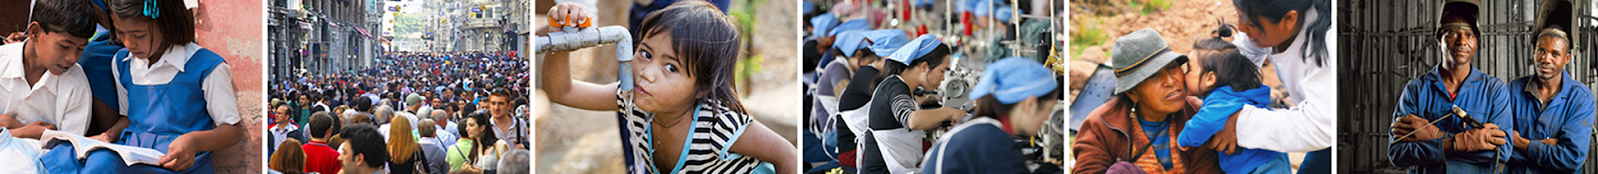
\includegraphics{ipums_banner.png}\\
Data Science for Social Scientists:\\
An applied course using IPUMS data }
\author{\textbf{Developed by:}\\
\hspace*{0.333em}\hspace*{0.333em}Daniel E. Ehrlich, \href{https://international.ipums.org/international/}{IPUMS, University of Minnesota}\\
\hspace*{0.333em}\hspace*{0.333em}Anna Tremblay, \href{https://www.clemson.edu/cbshs/departments/sacj/degrees/anthropology.html}{Dept of Soc, Anth, \& CJ, Clemson University}\\
\hspace*{0.333em}\hspace*{0.333em}Current Version compiled: 2023-01-04\\
\strut \\

\includegraphics[width=0.5\textwidth,height=\textheight]{ipums_i_logo.jpg}\\

\includegraphics[width=0.5\textwidth,height=\textheight]{clemson_logo.png}\\
\strut \\
\strut \\}
\date{}

\begin{document}
\maketitle

{
\setcounter{tocdepth}{1}
\tableofcontents
}
\hypertarget{preface}{%
\chapter*{Preface}\label{preface}}
\addcontentsline{toc}{chapter}{Preface}

An applied methods class for social scientists that uses real-world IPUMS data. This course is:

Open-source and customizable -\\
\hspace*{0.333em}\hspace*{0.333em}\hspace*{0.333em}All materials available on \href{https://github.com/ehrlichd/stats_book}{Github}\\
\strut \\
Made with open-source tools -\\
\hspace*{0.333em}\hspace*{0.333em}\href{https://cran.r-project.org/}{R}, \href{https://www.rstudio.com/products/rstudio/}{RStudio}, \href{https://bookdown.org/}{bookdown}\\
\strut \\
Driven by \textsuperscript{(nearly)} open-source data -\\
\hspace*{0.333em}\hspace*{0.333em}Harmonized across time and space: \href{https://ipums.org}{IPUMS}\\

\hypertarget{what-is-ipums}{%
\subsection*{What is IPUMS}\label{what-is-ipums}}
\addcontentsline{toc}{subsection}{What is IPUMS}

IPUMS started as a project to digitize the historical records of the US census.
It has expanded to include \href{https://www.ipums.org/}{9 data collections},
which are united in their methods and principles of making social science
research easier. IPUMS data consists of individual-level census and survey data
from more than 100 countries around the world. Notably:

\begin{itemize}
\tightlist
\item
  IPUMS \textbf{harmonizes} these data - ensuring consistently coded values across time and space.
\item
  IPUMS provides harmonized \textbf{GIS Shapefiles} for most census and survey data.
\item
  IPUMS provides extensive \textbf{metadata}, including:

  \begin{itemize}
  \tightlist
  \item
    Original questionnaire text.
  \item
    Universe definition and comparability statements.
  \item
    Alerts about notable changes in variable definition,
    universe, or coding schema
  \end{itemize}
\end{itemize}

IPUMS data is free to use for education and research purposes. Researchers need
only to register with an email address and brief project description. Nothing
too formal - we're just trying to understand what kinds of questions
researchers are interested in. For educators, we have additional resources
to facilitate set up of classroom accounts - making it easy to get your
students registered and share IPUMS data with them.

\hypertarget{why-make-this-course}{%
\subsection*{Why make this course}\label{why-make-this-course}}
\addcontentsline{toc}{subsection}{Why make this course}

In a world where information and data are increasingly accessible, it is of utmost importance for individuals to understand data science and the interpretation of data. We believe that education should be easily accessible and teaching resources should be freely available to aid in this endeavor. While we (DEE) may be slightly biased, we think IPUMS is a fantastic resource for both \textbf{Education} and \textbf{Research}. Real-world example datasets provide the bulk of the content for this course, providing an applied context we hope students (and instructors) will find engaging. We also know many instructors may be teaching across multiple disciplines, in large departments, or be the only ``data person'' at their institution. We think IPUMS data is useful to virtually any social science field. We provide some example lessons, and encourage instructors to develop their own, using our \texttt{lesson\_template.Rmd} to tailor this course to their subject or interest.

\hypertarget{getting-started}{%
\subsection*{Getting Started}\label{getting-started}}
\addcontentsline{toc}{subsection}{Getting Started}

In order to use this textbook, you will need to:

\begin{itemize}
\tightlist
\item
  download and install \href{https://posit.co/download/rstudio-desktop/}{RStudio}

  \begin{itemize}
  \tightlist
  \item
    This link also contains instructions and links to download \href{https://cran.rstudio.com/}{R from CRAN}
  \item
    Be sure you download the appropriate file for your Mac or PC
  \end{itemize}
\item
  Register for an with \href{https://ipums.org}{IPUMS} account. We provide \textbf{limited example data}, but in order take full advantage of these exercises:

  \begin{itemize}
  \tightlist
  \item
    \href{https://international.ipums.org/international-action/menu}{IPUMS registration for individuals}
  \item
    \href{https://international.ipums.org/international/classroom_accounts.shtml}{IPUMS registration for instructors}
  \end{itemize}
\end{itemize}

\hypertarget{course-description}{%
\section*{Course Description}\label{course-description}}
\addcontentsline{toc}{section}{Course Description}

This course is broken down into 3, 5-week units. Unit 1 focuses on familiarizing yourself with R and the IPUMS dataset. In Unit 2, each week will showcase a method/analysis using preselected variables. In class, students will walk through a given problem set and produce a lab report by the end of class. In Unit 3, students will work towards answering a research question that they pose, creating a research paper with literature review, data analysis, conclusion, and data outputs.

\hypertarget{course-aims}{%
\subsection*{Course Aims}\label{course-aims}}
\addcontentsline{toc}{subsection}{Course Aims}

Provide students with relevant, hands on, methodological training in data literacy and visualization.

\hypertarget{learning-outcomes}{%
\subsection*{Learning Outcomes}\label{learning-outcomes}}
\addcontentsline{toc}{subsection}{Learning Outcomes}

After this course, students will be able to:

\begin{itemize}
\tightlist
\item
  Understand the depth of the IPUMS database and the variables it has to\\
  offer
\item
  Compose R code to analyze the IPUMS data
\item
  Produce visually pleasing data outputs in R
\item
  Synthesize the information in a written report
\item
  Present the analysis in a poster format for other students
\end{itemize}

\hypertarget{guiding-principles}{%
\subsection*{Guiding Principles}\label{guiding-principles}}
\addcontentsline{toc}{subsection}{Guiding Principles}

\begin{itemize}
\tightlist
\item
  Phenomenon-based learning

  \begin{itemize}
  \tightlist
  \item
    try to start the class with a \textbf{question} or \textbf{problem}
  \item
    \emph{why} does the data look the way it does
  \item
    structure class so students work towards solving the problem
  \end{itemize}
\item
  Relevant examples

  \begin{itemize}
  \tightlist
  \item
    Drawn from multiple disciplines (eg, economics, demography)
  \item
    Can be added as modular examples/exercises
  \end{itemize}
\end{itemize}

\hypertarget{syllabus---general}{%
\section*{Syllabus - General}\label{syllabus---general}}
\addcontentsline{toc}{section}{Syllabus - General}

This syllabus is initially envisioned as 3 5-week sections. However, compilation and content are intended to be modular with templates for instructors to include their own specialties.

The basic structure of this course is:

\textbf{Unit 1 (Weeks 1-5):} Understanding and Testing Data

\begin{itemize}
\tightlist
\item
  Students use simple datasets bundled with the course or provided by the instructor.
\item
  Simplified data to illustrate trends.

  \begin{itemize}
  \tightlist
  \item
    EG: plotting continuous variable (AGE); Table of categorical variable (SEX); Crosstabs
  \end{itemize}
\end{itemize}

\textbf{Unit 2 (Weeks 6-10):} Finding Data and Asking Questions

\begin{itemize}
\tightlist
\item
  Students begin to analyze real world, IPUMS, datasets, provided by course/instructor.
\item
  Students begin to model real world phenomena

  \begin{itemize}
  \tightlist
  \item
    EG: SEX \textasciitilde{} EDUATTAIN ; SEX \textasciitilde{} EDATTAIN + EMPSTAT
  \end{itemize}
\item
  Students learn to perform exploratory analysis, hypothesis testing, and statistical inference.
\item
  Students learn to navigate IPUMS website,and find relevant data to thier research interest.
\end{itemize}

\textbf{Unit 3 (Weeks 11-15):} Discussing Data and Student Research

\begin{itemize}
\tightlist
\item
  Students develop a research question to be answered with IPUMS data.

  \begin{itemize}
  \tightlist
  \item
    Students are encouraged to fit it to their interests/major/discipline.
  \end{itemize}
\item
  Course time should be devoted to individual/small-group research.
\item
  Instructor/class present on recent research.

  \begin{itemize}
  \tightlist
  \item
    Instructor models constructive / scholarly criticism.
  \item
    Encourage students to critique published work - responsibly.
  \end{itemize}
\end{itemize}

\hypertarget{syllabus---detailed}{%
\section*{Syllabus - Detailed}\label{syllabus---detailed}}
\addcontentsline{toc}{section}{Syllabus - Detailed}

\hypertarget{unit-1-understanding-and-testing-data}{%
\subsection*{Unit 1 Understanding and Testing Data}\label{unit-1-understanding-and-testing-data}}
\addcontentsline{toc}{subsection}{Unit 1 Understanding and Testing Data}

Students become gain familiarity and comfortability navigating RStudio, coding in R and performing simple data manipulation and visualization exercises. Datasets in this section consist of real-world (or synthetic) data, but the focus is on understanding data types (EG: using Age as a continuous variable; sex, education, employment as categorical; etc). Instructors should acknowledge these as \textbf{educational} datasets and make explicit trends found within these data are devoid of context, and must be taken with a (rather large) grain of salt, if at all.

By the end of Unit 1, students will be able to:

\begin{itemize}
\tightlist
\item
  Download R and RStudio
\item
  Read data into R and
\item
  Write (save) data out of R
\item
  Summarize data visually

  \begin{itemize}
  \tightlist
  \item
    Using \texttt{base\ R}
  \item
    Using \texttt{ggplot} (tidyverse)
  \end{itemize}
\item
  Summarize data in tables

  \begin{itemize}
  \tightlist
  \item
    Using base R
  \item
    Using \texttt{gttable} / \texttt{tidyverse}
  \end{itemize}
\item
  Formally state and test assumptions of data

  \begin{itemize}
  \tightlist
  \item
    \emph{EG:} t-test, anova, correlations, regression
  \end{itemize}
\end{itemize}

By the end of Unit 1, students will understand

\begin{itemize}
\tightlist
\item
  Main types of data

  \begin{itemize}
  \tightlist
  \item
    \emph{EG:} logical, numeric, character, etc
  \item
    R specic vs general terms
  \end{itemize}
\item
  How to create and describe various data distributions

  \begin{itemize}
  \tightlist
  \item
    \emph{EG:} normal, poisson, normal-skewed, etc
  \end{itemize}
\item
  Know which types statistical tests are appropriate for a given set of data.
\end{itemize}

\hypertarget{week-1-intro-to-r-data-types-data-structures}{%
\subsubsection*{Week 1: Intro to R, data types, data structures}\label{week-1-intro-to-r-data-types-data-structures}}
\addcontentsline{toc}{subsubsection}{Week 1: Intro to R, data types, data structures}

\hypertarget{week-2-plotting-data-distributions}{%
\subsubsection*{Week 2: Plotting Data, Distributions}\label{week-2-plotting-data-distributions}}
\addcontentsline{toc}{subsubsection}{Week 2: Plotting Data, Distributions}

\hypertarget{week-3-statisitcal-testing-of-simple-data-sets}{%
\subsubsection*{Week 3: Statisitcal testing of simple data sets}\label{week-3-statisitcal-testing-of-simple-data-sets}}
\addcontentsline{toc}{subsubsection}{Week 3: Statisitcal testing of simple data sets}

\hypertarget{week-4-correlation-and-relationships-of-simple-data-sets}{%
\subsubsection*{Week 4: Correlation and Relationships of simple data sets}\label{week-4-correlation-and-relationships-of-simple-data-sets}}
\addcontentsline{toc}{subsubsection}{Week 4: Correlation and Relationships of simple data sets}

\hypertarget{week-5-tbd}{%
\subsubsection*{Week 5: (TBD)}\label{week-5-tbd}}
\addcontentsline{toc}{subsubsection}{Week 5: (TBD)}

\hypertarget{unit-2-finding-data-and-asking-questions-using-ipums-data}{%
\subsection*{Unit 2 Finding Data and Asking Questions (Using IPUMS Data)}\label{unit-2-finding-data-and-asking-questions-using-ipums-data}}
\addcontentsline{toc}{subsection}{Unit 2 Finding Data and Asking Questions (Using IPUMS Data)}

Here we demonstrate two \textbf{different} approaches to conducting research. Students become familiar writing up short lab reports detailing their findings. For Section \ref{exploratory}, we/instructor provides students with simple datasets from IPUMS (or other real-world data). Students will learn exploratory data analysis techniques and how to create lab reports to summarize key findings.

For unit \ref{hypothesis}, students will learn to develop their own simple research questions or social-science hypotheses. They will seek out data to answer these questions, learning to navigate \href{https://ipums.org}{ipums.org}, and create \textbf{data extracts}, as well as hypothesis-testing statistical methods. Again, lab reports to summarize findings.

\hypertarget{week-6-intro-to-ipums}{%
\subsubsection{Week 6: Intro to IPUMS}\label{week-6-intro-to-ipums}}

\hypertarget{week-7-exploratory-analysis}{%
\subsubsection*{Week 7: Exploratory analysis}\label{week-7-exploratory-analysis}}
\addcontentsline{toc}{subsubsection}{Week 7: Exploratory analysis}

If you've just collected a survey, or other raw data, you may not know what you're looking for. This is perfectly ok but goes against \emph{the scientific method} most people learned in grade school.

This unit begins by presenting data/distributions and asking students to begin interpreting the data . visual exploration is encouraged and basic of data manipulation are taught
* \emph{EG:} how to subset data, how to reshape data, how to re-code data, how to convert from one \texttt{data\ type} to another.

Example lab exercise:

Students given a data set (xls, csv, etc)
* load data, perform manipulations, basic summaries
+ cross tabs
+ group means by a covariate
* inspect data visually
+ \emph{DESCRIBE} the distribution - is it normal? significant?
* \emph{FIND} aquestion in the spread of the data
+ how can you test this (maybe small group work)
* write up/ present results
+ think on confounding factors / biases

\hypertarget{week-8-hypothesis-testing}{%
\subsubsection*{Week 8: Hypothesis Testing}\label{week-8-hypothesis-testing}}
\addcontentsline{toc}{subsubsection}{Week 8: Hypothesis Testing}

If, on the other hand you have an a pre-existing idea you want to test. We can follow the traditional \emph{scientific method}. With a question in mind, the first question is: where to look. What better place than \href{https://ipums.org}{IPUMS}!

Begin introducing navigation of web resources - mainly IPUMS international

Students should become comfortable working through lab exercises:
* Define a question (or be presented with one)
* Download variables from IPUMS (course downloads possible)
* Perform a basic analysis (discussed in Unit 1)
* Generate a \textbf{visual argument} for your analysis
+ Include explanation/interpretation/reflection on the question at hand, and the data used
+ Any obvious biases
+ Any obvious confounding factors

\hypertarget{week-9-statistical-inference}{%
\subsubsection*{Week 9: Statistical Inference}\label{week-9-statistical-inference}}
\addcontentsline{toc}{subsubsection}{Week 9: Statistical Inference}

\hypertarget{week-10-tbd}{%
\subsubsection*{Week 10: (TBD)}\label{week-10-tbd}}
\addcontentsline{toc}{subsubsection}{Week 10: (TBD)}

\hypertarget{unit-3-discussing-data-and-student-research}{%
\subsection*{Unit 3 Discussing Data and Student Research}\label{unit-3-discussing-data-and-student-research}}
\addcontentsline{toc}{subsection}{Unit 3 Discussing Data and Student Research}

Students will select their own research question that can be answered with the IPUMS data set and will spend five weeks conducting a research project complete with data analysis, visualization, and interpretation.

In this section we encourage the instructor to provide ample time for independent student/small-group research. Some class time should be devoted to modeling healthy discussion and critique of methods. Students should learn to discuss not just \emph{how} to answer a research question but \emph{why} they are asking/answering it. What impact does the question/answers have. Is the question releveant/meaningful, and importantly, Is this research question perpetuating racist ideas.

We provide some examples here but encourage instructors (or students) to bring in recent journal/popular articles that do (or do not) apply data science methods well.

\hypertarget{week-11-students-develop-research-question}{%
\subsubsection*{Week 11: Students develop research Question}\label{week-11-students-develop-research-question}}
\addcontentsline{toc}{subsubsection}{Week 11: Students develop research Question}

\hypertarget{week-12-students-find-relevant-variables-from-ipums}{%
\subsubsection*{Week 12: Students find relevant variables from IPUMS}\label{week-12-students-find-relevant-variables-from-ipums}}
\addcontentsline{toc}{subsubsection}{Week 12: Students find relevant variables from IPUMS}

\hypertarget{week-13-students-test-and-evaluate-results}{%
\subsubsection*{Week 13: Students test and evaluate results}\label{week-13-students-test-and-evaluate-results}}
\addcontentsline{toc}{subsubsection}{Week 13: Students test and evaluate results}

\hypertarget{week-14-students-prepare-presentations-of-results}{%
\subsubsection*{Week 14: Students prepare presentations of results}\label{week-14-students-prepare-presentations-of-results}}
\addcontentsline{toc}{subsubsection}{Week 14: Students prepare presentations of results}

\hypertarget{week-15-students-present-work-slides-poster-podium-etc}{%
\subsubsection*{Week 15: Students present work (slides, poster, podium, etc)}\label{week-15-students-present-work-slides-poster-podium-etc}}
\addcontentsline{toc}{subsubsection}{Week 15: Students present work (slides, poster, podium, etc)}

\hypertarget{dev-notes}{%
\chapter*{DEV NOTES}\label{dev-notes}}

\hypertarget{to-do}{%
\subsection*{TO DO}\label{to-do}}
\addcontentsline{toc}{subsection}{TO DO}

\begin{itemize}
\item
  \textbf{UPDATE TODO LIST}
\item
  Make chapter 1 chapter 2
\item
  Anna Adds chapter con data science intro exclusive of R/IPUMS
\item
  discuss style

  \begin{itemize}
  \tightlist
  \item
    key terms section for each chapter?
  \item
    key terms in \textbf{bold}
  \item
    italics for \emph{emphasis}
  \item
    are we pro-hyphens, or are they pedantic?
  \end{itemize}
\end{itemize}

\hypertarget{misc-ideas}{%
\subsection*{MISC IDEAS}\label{misc-ideas}}
\addcontentsline{toc}{subsection}{MISC IDEAS}

\begin{itemize}
\tightlist
\item
  Application forward
\item
  Present research/ analysis/results FIRST, then explain the mathematical principals behind it
\item
  daily/weekly ``i'm stuck on\ldots{}''

  \begin{itemize}
  \tightlist
  \item
    Students send in questions (night before class) and instructor spends 10-15 mins talking through (or collaboratively working through with class) solutions
  \item
    Alternatively, once a month maybe a longer class covering ``common problems asked this month''
    daily/weekly ``recent research''
  \end{itemize}
\item
  pick out a recent article with good visualization (or bad) and spend 5-10 mins discussing what makes it good (or bad)

  \begin{itemize}
  \tightlist
  \item
    Encourage students to find articles for extra credit
  \end{itemize}
\end{itemize}

\hypertarget{documentation}{%
\subsection*{Documentation}\label{documentation}}
\addcontentsline{toc}{subsection}{Documentation}

This function grabs any packages in your project and adds them to a local list that can be referenced using \texttt{R-pacakgename}
* \textbf{NOTE} in practice, that needs to be wrapped in markdown syntax, eg:
\texttt{{[}@R-bookdown{]}}
* See help files for more info - might be able to create/add a \texttt{citation} file

\hypertarget{unit-1-the-basics}{%
\chapter*{Unit 1: The Basics}\label{unit-1-the-basics}}
\addcontentsline{toc}{chapter}{Unit 1: The Basics}

\hypertarget{lesson-0}{%
\section*{Lesson 0:}\label{lesson-0}}

Lesson 0 files should contain a brief summary of the topics within each unit

Lesson 0 can also be used for a brainstorming space to sketch out ideas before creating \texttt{Unit\#\_Lesson\#} files.

\hypertarget{lesson-1-what-is-data-collecting-visualizing-data}{%
\section*{Lesson 1: What IS Data / Collecting / Visualizing Data}\label{lesson-1-what-is-data-collecting-visualizing-data}}

\hypertarget{lesson-2-intro-to-r-data-types-data-structures}{%
\section*{Lesson 2: Intro to R, data types, data structures}\label{lesson-2-intro-to-r-data-types-data-structures}}

\hypertarget{lesson-3-comparing-data}{%
\section*{Lesson 3: Comparing Data}\label{lesson-3-comparing-data}}

\hypertarget{lesson-4}{%
\section*{Lesson 4:}\label{lesson-4}}

\hypertarget{lesson-5}{%
\section*{Lesson 5:}\label{lesson-5}}

\hypertarget{unit-wide-glossary}{%
\section*{Unit-wide Glossary}\label{unit-wide-glossary}}
\addcontentsline{toc}{section}{Unit-wide Glossary}

\emph{Is this redundant?}

\hypertarget{what-is-data}{%
\chapter{\texorpdfstring{What \emph{is} data?}{What is data?}}\label{what-is-data}}

\hypertarget{pov}{%
\section{POV:}\label{pov}}

\begin{quote}
In a social science class, your teacher tells you that the CDC
reports average male height in the United States to be 69
inches or 5ft 9in. While browsing dating apps, you notice that
nearly all the men report that they are 6ft or over. You wonder
if this is a bias in reporting, or if the area where you live
and attend college has significantly taller men. To test your
theory, you want to collect data on height from individuals in
your data science class to test if males are truly taller on campus
than the country average.

\textbf{Source:} \url{https://www.cdc.gov/nchs/fastats/body-measurements.htm}**
\end{quote}

\hypertarget{activity---collect-data-on-height}{%
\subsection{ACTIVITY - collect data on height}\label{activity---collect-data-on-height}}

\textbf{If in-person}
* Create a histogram (x axis) on a blackboard/wall, have students place their heights
with a post-it note
+ Start with one distribution for whole class
+ Repeat with separate distributions for M/F
+ \emph{DEE: I want to find a way to acknowledge this dichotomy ignores non-binary individuals, and include some suggestions on how to discuss it.}

\hypertarget{activity---collect-data-on-birth-month}{%
\subsection{ACTIVITY - collect data on birth month}\label{activity---collect-data-on-birth-month}}

\begin{itemize}
\tightlist
\item
  Create a histogram (x axis) on a blackboard/wall, have students place their heights
  with a post-it note

  \begin{itemize}
  \tightlist
  \item
    Students place post-it notes on month of birth
  \end{itemize}
\end{itemize}

\textbf{IDEALLY:} Have both a histogram of height AND histogram of birth month visible
at the same time. Compare/contrast distributions of the two data sets.

\hypertarget{explore}{%
\section{Explore}\label{explore}}

Questions to consider:
* \emph{Why do we plot data}
* \emph{What does the} \textbf{distribution} \emph{of post-it notes look like?}
* \emph{What can you infer from the distribution(s)}
* \emph{How does the distribution of height differ from birth month?}

\hypertarget{example-datasets}{%
\subsection{Example Datasets}\label{example-datasets}}

If you're working through this course on your own, or are unable to facilitate a classroom activity, see the companion R package, \texttt{ipumsED}, which includes example data sets for each lesson, as well as custom code and functions to facilitate learning data science with IPUMS data.

\emph{DEE: This could probably be stated at the begining of unit 1}

\hypertarget{activity---calculate-by-hand}{%
\subsection{ACTIVITY - Calculate by hand}\label{activity---calculate-by-hand}}

In our hypothetical setup, we are interested in the \textbf{average} height.
* \emph{What does it mean to be} \textbf{\emph{average}}
* \emph{Which height would you say is average? (eyeballing)}
* \emph{Which Birth Month would you say is average? - is there one?}

Write out steps for calculating \textbf{mean} - trivial as it may seem.

\hypertarget{explain}{%
\section{Explain}\label{explain}}

In the context of this example, we \textbf{collected} data on height and birth month for individuals in our class.
Plotting our data allows us to \textbf{visualize} the data, making it easy to interpret.

\hypertarget{ellaborate}{%
\section{Ellaborate}\label{ellaborate}}

\hypertarget{so-what-is-data}{%
\subsection{So what is data?}\label{so-what-is-data}}

Data is defined as ``facts and statistics collected together for
reference or analysis.''\footnote{This is from the internet and needs to
  be our words} As seen in Figure 1.1, there are two types of data:
quantitative and qualitative. \textbf{Quantitative data} are able to
be expressed in numerical format and are countable. These data
are either discrete or continuous where \textbf{discrete data} uses
numeric bins. For example, we use our age as discrete
quantitative data, we round our age to the previous year (eg.,
20, 21, 22). \textbf{Continuous data} does not use bins, but rather
includes all of the fractions between two whole numbers. An
example could be most physical measures like height, weight, the
speed at which an individual runs.

\textbf{Qualitative data} describes characteristics or categories and
can be broken down into two categories, nominal or ordinal.
\textbf{Nominal data} has no inherent ordering but it can be
categorized. Examples include country or origin, gender, hair
color, race, etc. \textbf{Ordinal data} can both be categorized and
ordered (e.g., first, second, and third place is a race).

\begin{quote}
Going back to our hypothesis of male height on campus, heights
are continuous, qualitative data. It is difficult for people to
report their specific height and you assume that most
individuals will report it rounded to the closest inch. This
makes the data you will actually use, discrete quantitative
data.
\end{quote}

\hypertarget{collecting-data}{%
\subsection{Collecting Data}\label{collecting-data}}

The first step to answering a research question is to collect
your data. Broadly, data comes in two forms, primary and
secondary. (Fig 1.2) \textbf{Primary data} is data that is collected
directly by the researcher. Surveys, observations,
experimentation, questionnaires, and interviews are all examples
of primary data. \textbf{Secondary data} is collected from published
or unpublished literature. It is collected by different
researchers and compiled for use by a second scientist. This type
of data includes data found in published articles, books,
journals, biographies, and government records like the US Census.

Once compiled, you now have a data set which is comprised of
observations and variables. An \textbf{observation} is all of the
measures taken for one person or item. A \textbf{variable} is what is
being measured.

\begin{quote}
The US CDC data is secondary, but you are collecting height
data yourself in class as a comparison. The survey or
questionnaire you use on your classmates is primary data. Each
individual is an observation and the variable of interest is
height.
\end{quote}

\hypertarget{populations-and-sampling}{%
\subsection{POPULATIONS AND SAMPLING}\label{populations-and-sampling}}

\textbf{Random Sampling:} It is a sampling method in which all the
items have an equal chance of being selected and the individuals
who are selected are just like the ones who are not selected

\textbf{Stratified Random Sampling:} It is a process to gather data by
separating the actual population into the distinct subset or
strata, and then choosing simple random samples from each stratum
Your research question is about the height of all males at your
college, but recording height data for each individual would be
very difficult and time consuming. You instead decide to use a
sample of males in your data science class. This is a random
sample as each male individual has an equally likely chance of
being samples (that is, unless a prerequisite exists).

Sampling strategy can lead to \textbf{bias}

\begin{quote}
If you had chosen a different sample, like the men's basketball
team, your results would have been biased.
\end{quote}

\hypertarget{evaluation}{%
\section{Evaluation}\label{evaluation}}

\hypertarget{review-questions}{%
\subsection{Review Questions}\label{review-questions}}

\begin{itemize}
\tightlist
\item
  What is one example of collecting/visualizing data from your own life
\item
  Is height a \textbf{continuous} or \textbf{discrete} variable and Why?
\end{itemize}

\hypertarget{exercises}{%
\subsection{Exercises}\label{exercises}}

Brainstorm 3 topics/questions that are of interest to you personally, or academically.
* What \textbf{variable(s)} will you need to collect to study this phenomenon?
* Describe these variable(s), are they qualitative or quantitative? Continuous or ordinal?

\hypertarget{glossary}{%
\section*{Glossary}\label{glossary}}
\addcontentsline{toc}{section}{Glossary}

\hypertarget{intro-to-r-data-types-data-structures}{%
\chapter{Intro to R, data types, data structures}\label{intro-to-r-data-types-data-structures}}

In the previous lesson, we began thinking about \textbf{data}, how to talk about it,
and how to \textbf{visualize} it. We also talked about one type of average, the \textbf{mean.}

\hypertarget{engage}{%
\section{Engage}\label{engage}}

\emph{What do you think the following code does?}

\begin{Shaded}
\begin{Highlighting}[]
\NormalTok{my\_data }\OtherTok{\textless{}{-}} \FunctionTok{read\_excel}\NormalTok{(}\StringTok{"//filepath/directory/filename.xlsx"}\NormalTok{)}
\end{Highlighting}
\end{Shaded}

\emph{Hint:} There are 4 ``things'' in the above code:
\texttt{my\_data},
\texttt{\textless{}-},
\texttt{read\_excel()},
\texttt{//filepath/directory/filename.xlsx}

\hypertarget{r-vs-rstudio}{%
\subsection{R vs RStudio}\label{r-vs-rstudio}}

\begin{itemize}
\item
  If \texttt{R} is the engine, then \texttt{RStudio} is the car.
\item
  If \texttt{R} is the text, Rstudio is the text-editor.
\item
  \texttt{R} is the \textbf{programming language}, \texttt{Rstudio} is the \textbf{Integrated Development Environment (IDE)}.

  \begin{itemize}
  \tightlist
  \item
    \emph{What do you think some differences are between R and RStudio?}
  \end{itemize}
\end{itemize}

\texttt{RStudio} is a program/app just like Google Chrome or Microsoft Word. Each
of these programs provide a \textbf{Graphical User Interface (GUI)}, a pretty way for
a user to use a mouse and keyboard to do \emph{something.}

An \textbf{IDE} is a special kind of program/app that provides MANY tools for writing and running code.

\hypertarget{orientation-to-rstudio}{%
\subsection{Orientation to RStudio}\label{orientation-to-rstudio}}

\emph{SUGGESTION: Instructor live demos interacting with RStudio while students follow along on computers}

When you first open RStudio, you'll see 3 \textbf{panes}, all of which will look fairly empty at the moment.

If you're using the default layout, you should see:
* On the left, the \texttt{Console} \textbf{pane}
* On the Top-right, the \texttt{Environment} \textbf{pane}
* On the Bottom-right, the \texttt{Files} \textbf{pane}

A keen eye will also notice that each of these \textbf{panes} contains multiple \textbf{tabs}. We will go over the uses of many of these \textbf{tabs}, but for now let's start with \texttt{Console.}

The \texttt{Console} is where you input \texttt{R\ code}, run it, and see the results.

At it's simplest \texttt{RStudio} is a calculator. Try typing \texttt{4\ +\ 4} into the \texttt{Console},
then press the \texttt{{[}Enter{]}} key to run the code. Immediately, \texttt{R} prints the result as we see here:

\begin{Shaded}
\begin{Highlighting}[]
\DecValTok{4} \SpecialCharTok{+} \DecValTok{4}
\end{Highlighting}
\end{Shaded}

\begin{verbatim}
## [1] 8
\end{verbatim}

The \texttt{Console} serves as a running log of all your operations for your current session, but it can be helpful to temporarily save your results as \texttt{R\ objects}. We do this using the \textbf{assignment operator} we saw earlier: \texttt{\textless{}-}

\begin{Shaded}
\begin{Highlighting}[]
\NormalTok{answer }\OtherTok{\textless{}{-}} \DecValTok{4}\SpecialCharTok{+}\DecValTok{4}
\end{Highlighting}
\end{Shaded}

By default, \texttt{Console} only prints results if they have no where else to go. If they're stored as an \texttt{Robject}, no result is printed, but you should now see \texttt{answer} listed in the \texttt{Environment} \textbf{pane}.

\hypertarget{explore---interacting-with-r-objects}{%
\section{Explore - Interacting with R objects}\label{explore---interacting-with-r-objects}}

\hypertarget{load-the-data}{%
\subsection{Load the Data}\label{load-the-data}}

\begin{Shaded}
\begin{Highlighting}[]
\NormalTok{dir\_path }\OtherTok{\textless{}{-}} \FunctionTok{file.path}\NormalTok{(}\StringTok{"inst"}\NormalTok{,}\StringTok{"unit1\_data"}\NormalTok{)}
\NormalTok{survey\_path }\OtherTok{\textless{}{-}} \FunctionTok{file.path}\NormalTok{(dir\_path, }\StringTok{"data\_template.xlsx"}\NormalTok{)}

\NormalTok{data }\OtherTok{\textless{}{-}}\NormalTok{ readxl}\SpecialCharTok{::}\FunctionTok{read\_excel}\NormalTok{(survey\_path)}
\end{Highlighting}
\end{Shaded}

What is \texttt{data}?? Below we call the \texttt{class()} function on \texttt{data} and see that it has 3 classes:
\texttt{tbl\_df} , \texttt{tbl} , \texttt{data.frame}

The first two classes, \texttt{tbl\_df,\ tbl} indicate it is a special kind of table, in the \texttt{tibble} format. In general, you can interact with these like a \texttt{matrix} or \texttt{data.frame} but they have additional features.

\begin{Shaded}
\begin{Highlighting}[]
\FunctionTok{class}\NormalTok{(data)}
\end{Highlighting}
\end{Shaded}

\begin{verbatim}
## [1] "tbl_df"     "tbl"        "data.frame"
\end{verbatim}

We can call \texttt{colnames()} on data, like a regular \texttt{data.frame} or \texttt{matrix}. Or we can take advantage of the \texttt{tibble} structure and use the \texttt{glimpse()} function which provides a succinct summary of your data.

\begin{Shaded}
\begin{Highlighting}[]
\FunctionTok{colnames}\NormalTok{(data)}
\end{Highlighting}
\end{Shaded}

\begin{verbatim}
## [1] "individual"    "Birth_Month"   "Height_inches"
\end{verbatim}

\begin{Shaded}
\begin{Highlighting}[]
\NormalTok{tibble}\SpecialCharTok{::}\FunctionTok{glimpse}\NormalTok{(data)}
\end{Highlighting}
\end{Shaded}

\begin{verbatim}
## Rows: 32
## Columns: 3
## $ individual    <dbl> 1, 2, 3, 4, 5, 6, 7, 8, 9, 10, 11, 12, 13, 14, 15, 16, 1~
## $ Birth_Month   <chr> "January", "September", "March", "April", "April", "Octo~
## $ Height_inches <dbl> 70, 64, 72, 61, 55, 65, 72, 75, 69, 75, 76, 70, 70, 69, ~
\end{verbatim}

\hypertarget{inspect-the-data}{%
\subsection{Inspect the Data}\label{inspect-the-data}}

What is \texttt{data}?? Below we call the \texttt{class()} function on \texttt{data} and see that it has 3 classes:
\texttt{tbl\_df} , \texttt{tbl} , \texttt{data.frame}

The first two classes, \texttt{tbl\_df,\ tbl} indicate it is a special kind of table, in the \texttt{tibble} format. In general, you can interact with these like a \texttt{matrix} or \texttt{data.frame} but they have additional features.

\begin{Shaded}
\begin{Highlighting}[]
\FunctionTok{class}\NormalTok{(data)}
\end{Highlighting}
\end{Shaded}

\begin{verbatim}
## [1] "tbl_df"     "tbl"        "data.frame"
\end{verbatim}

We can call \texttt{colnames()} on data, like a regular \texttt{data.frame} or \texttt{matrix}. Or we can take advantage of the \texttt{tibble} structure and use the \texttt{glimpse()} function which provides a succinct summary of your data.

\begin{Shaded}
\begin{Highlighting}[]
\FunctionTok{colnames}\NormalTok{(data)}
\end{Highlighting}
\end{Shaded}

\begin{verbatim}
## [1] "individual"    "Birth_Month"   "Height_inches"
\end{verbatim}

\begin{Shaded}
\begin{Highlighting}[]
\NormalTok{tibble}\SpecialCharTok{::}\FunctionTok{glimpse}\NormalTok{(data)}
\end{Highlighting}
\end{Shaded}

\begin{verbatim}
## Rows: 32
## Columns: 3
## $ individual    <dbl> 1, 2, 3, 4, 5, 6, 7, 8, 9, 10, 11, 12, 13, 14, 15, 16, 1~
## $ Birth_Month   <chr> "January", "September", "March", "April", "April", "Octo~
## $ Height_inches <dbl> 70, 64, 72, 61, 55, 65, 72, 75, 69, 75, 76, 70, 70, 69, ~
\end{verbatim}

\hypertarget{summarize-data}{%
\section*{Summarize Data}\label{summarize-data}}
\addcontentsline{toc}{section}{Summarize Data}

\hypertarget{continuous-data}{%
\subsection*{Continuous Data}\label{continuous-data}}
\addcontentsline{toc}{subsection}{Continuous Data}

For continuous data, we often want to summarize our data by describing the \textbf{mean, median, and/or range}. \textbf{Mean} and \textbf{median} describe the \emph{central tendency} of the data, while \textbf{range} describes the full extant of the data, as seen below.

NOTE: if \texttt{NA} are present in the data, be sure to use the \texttt{na.rm=TRUE} flag for these operations.

\begin{Shaded}
\begin{Highlighting}[]
\FunctionTok{mean}\NormalTok{(data}\SpecialCharTok{$}\NormalTok{Height\_inches, }\AttributeTok{na.rm =}\NormalTok{ T)}
\end{Highlighting}
\end{Shaded}

\begin{verbatim}
## [1] 66.5625
\end{verbatim}

\begin{Shaded}
\begin{Highlighting}[]
\FunctionTok{median}\NormalTok{(data}\SpecialCharTok{$}\NormalTok{Height\_inches, }\AttributeTok{na.rm =}\NormalTok{ T)}
\end{Highlighting}
\end{Shaded}

\begin{verbatim}
## [1] 66.5
\end{verbatim}

\begin{Shaded}
\begin{Highlighting}[]
\FunctionTok{range}\NormalTok{(data}\SpecialCharTok{$}\NormalTok{Height\_inches, }\AttributeTok{na.rm =}\NormalTok{ T)}
\end{Highlighting}
\end{Shaded}

\begin{verbatim}
## [1] 55 76
\end{verbatim}

\hypertarget{all-in-summary}{%
\subsection*{All in summary()}\label{all-in-summary}}
\addcontentsline{toc}{subsection}{All in summary()}

\textbf{Mean}, \textbf{median}, and \textbf{range} will all be reported by calling \texttt{summary()} on a \texttt{numeric\ vector}, such as \texttt{Height\_inches}. In addition, the lower and upper quartiles will be reported, along with the number of \texttt{NA} responses.

NOTE: \texttt{summary()} does NOT require special handling for \texttt{NA} values, in fact - it expects them!

\begin{Shaded}
\begin{Highlighting}[]
\FunctionTok{summary}\NormalTok{(data}\SpecialCharTok{$}\NormalTok{Height\_inches)}
\end{Highlighting}
\end{Shaded}

\begin{verbatim}
##    Min. 1st Qu.  Median    Mean 3rd Qu.    Max. 
##   55.00   64.00   66.50   66.56   70.00   76.00
\end{verbatim}

\hypertarget{mode}{%
\section{Mode}\label{mode}}

You're probably familiar with \textbf{mean} and \textbf{median} being talked about with a
third term, \textbf{mode}. The \textbf{mode} is the most commonly occuring value in a
dataset. It's often important to know the \textbf{modal response} of survey data.
While a commonly reported metric(??), there is no \texttt{mode()} function included in
\texttt{base\ r}\ldots{}

so we'll just have to create our own!

\hypertarget{mode-code}{%
\subsection{Mode Code}\label{mode-code}}

One common measure of data reported is the mode, or most frequently occuring value. For whatever reason, this is not a default function in R, but we can easily write our own function like so:

\begin{Shaded}
\begin{Highlighting}[]
\NormalTok{my\_mode }\OtherTok{\textless{}{-}} \ControlFlowTok{function}\NormalTok{(x)\{}
\NormalTok{  tt }\OtherTok{\textless{}{-}} \FunctionTok{table}\NormalTok{(x) }\DocumentationTok{\#\# find frequencies}
\NormalTok{  tt }\OtherTok{\textless{}{-}}\NormalTok{ tt[}\FunctionTok{order}\NormalTok{(tt, }\AttributeTok{decreasing =} \ConstantTok{TRUE}\NormalTok{)] }\DocumentationTok{\#\# resort based on freq}
  
  \DocumentationTok{\#\# check number of modes}
\NormalTok{  max }\OtherTok{\textless{}{-}} \FunctionTok{max}\NormalTok{(tt)}
\NormalTok{  n\_max }\OtherTok{\textless{}{-}} \FunctionTok{sum}\NormalTok{(tt}\SpecialCharTok{==}\NormalTok{max)}
  
  
  \ControlFlowTok{if}\NormalTok{(n\_max }\SpecialCharTok{\textgreater{}} \DecValTok{1}\NormalTok{ )\{}
    \FunctionTok{warning}\NormalTok{(}\StringTok{"More than one mode detected"}\NormalTok{)}
    \FunctionTok{return}\NormalTok{(tt[tt}\SpecialCharTok{==}\NormalTok{max])}
\NormalTok{  \} }\ControlFlowTok{else}\NormalTok{ \{}
    \DocumentationTok{\#\# return only the first value}
    \FunctionTok{return}\NormalTok{(tt[}\DecValTok{1}\NormalTok{]) }\DocumentationTok{\#\# return whatever the highrst frequency is}
\NormalTok{  \}}

  
\NormalTok{\}}
\end{Highlighting}
\end{Shaded}

\hypertarget{mode-results}{%
\subsection{Mode Results}\label{mode-results}}

Now that we've created out own \texttt{function}, it's easy to find the \textbf{mode}

\begin{Shaded}
\begin{Highlighting}[]
\FunctionTok{my\_mode}\NormalTok{(data}\SpecialCharTok{$}\NormalTok{Height\_inches)}
\end{Highlighting}
\end{Shaded}

\begin{verbatim}
## Warning in my_mode(data$Height_inches): More than one mode detected
\end{verbatim}

\begin{verbatim}
## x
## 64 65 69 70 
##  4  4  4  4
\end{verbatim}

\hypertarget{visualizing-data}{%
\section{Visualizing Data}\label{visualizing-data}}

The above summaries describe data with numbers, but we can also describe data visually.

\hypertarget{continuous-data---boxplots}{%
\subsection{Continuous Data - Boxplots}\label{continuous-data---boxplots}}

Univariate continuous data, like height, can be visualized using a box and whisker plot, which shows many of the components of summary:

\begin{itemize}
\tightlist
\item
  the \textbf{median} is the black bar in the middle
\item
  the \textbf{quartiles} (25th and 75th percentiles) are represented by the extents of the boxes
\item
  The \textbf{range} is shown by the whiskers, with outliers shown indvidually, if needed.
\end{itemize}

\begin{Shaded}
\begin{Highlighting}[]
\FunctionTok{boxplot}\NormalTok{(data}\SpecialCharTok{$}\NormalTok{Height\_inches)}
\end{Highlighting}
\end{Shaded}

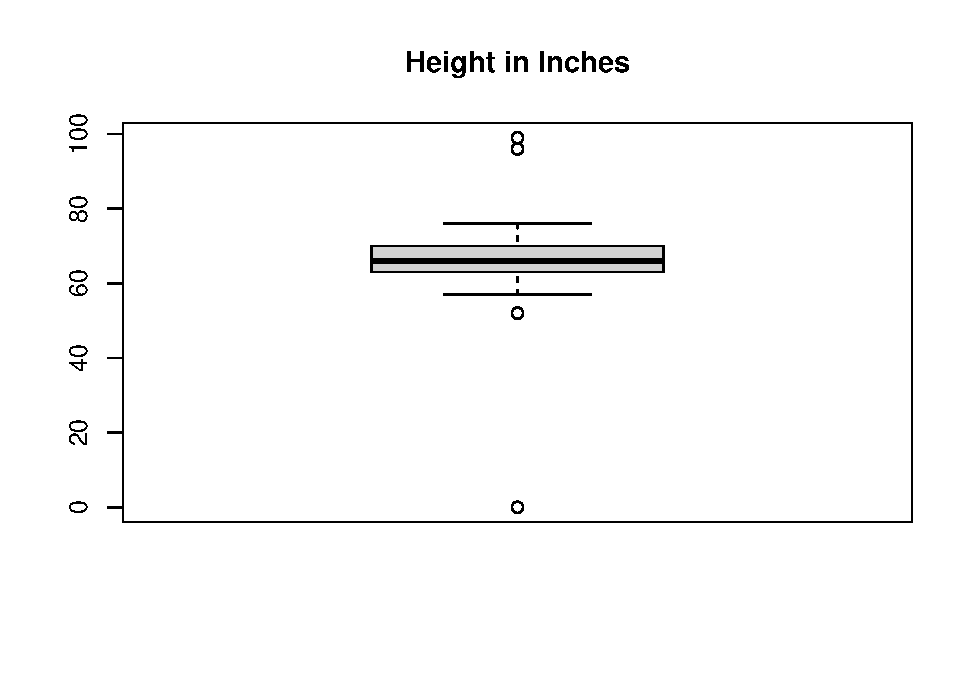
\includegraphics{_main_files/figure-latex/unnamed-chunk-14-1.pdf}

\hypertarget{continuous-data---histograms}{%
\subsection{Continuous Data - Histograms}\label{continuous-data---histograms}}

Continuous data, can also be broken into \textbf{bins} and plotted as a \textbf{histogram}. The \texttt{hist()} function will attempt to find the optimum number of bins for you, but you can specify a different number with the \texttt{breaks} argument.

\begin{Shaded}
\begin{Highlighting}[]
\FunctionTok{hist}\NormalTok{(data}\SpecialCharTok{$}\NormalTok{Height\_inches, }\AttributeTok{main =} \StringTok{"Histogram of Height"}\NormalTok{, }\AttributeTok{xlab =} \StringTok{"Height (in)"}\NormalTok{)}
\end{Highlighting}
\end{Shaded}

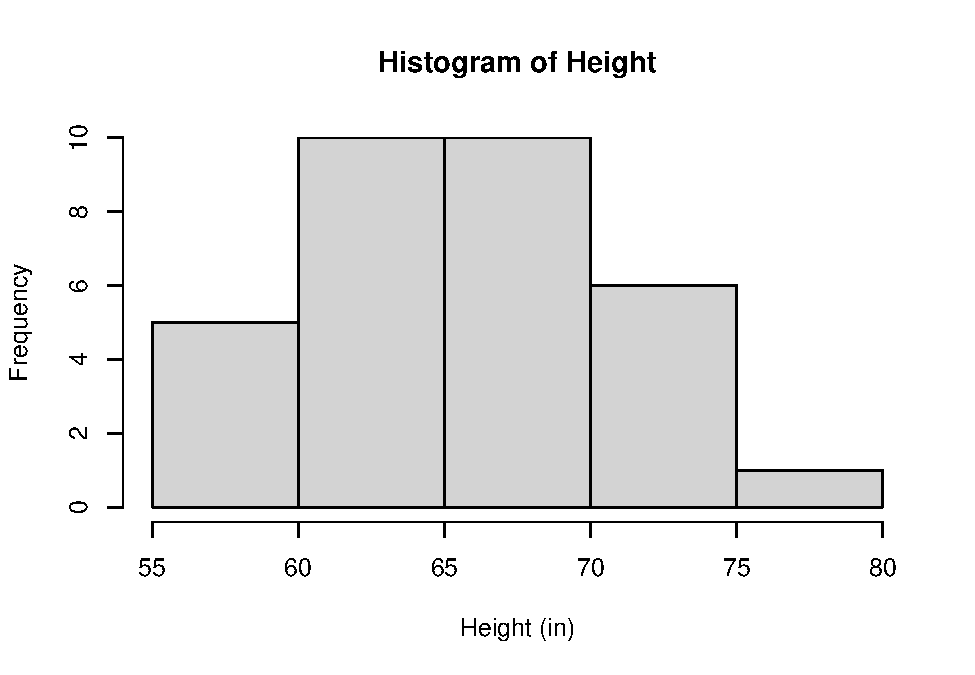
\includegraphics{_main_files/figure-latex/unnamed-chunk-15-1.pdf}

\hypertarget{categorical-data}{%
\subsection{Categorical Data}\label{categorical-data}}

Categorical data is already in discrete units. In general with categorical data, we want to count the \textbf{frequency} of unique values. There are many ways to do this, but one of the easiest is the \texttt{table()} function. Saving the results of the table to an object, \texttt{birth\_freq}, allows you to save and print the results at any time.

\begin{Shaded}
\begin{Highlighting}[]
\NormalTok{birth\_freq }\OtherTok{\textless{}{-}} \FunctionTok{table}\NormalTok{(data}\SpecialCharTok{$}\NormalTok{Birth\_Month)}

\NormalTok{birth\_freq}
\end{Highlighting}
\end{Shaded}

\begin{verbatim}
## 
##     April    August  December  February   January      July      June     March 
##         4         2         3         1         3         2         3         2 
##       May  November   October September 
##         4         4         2         2
\end{verbatim}

We can also visualize our tabulated results using a \textbf{barplot} as below.

\begin{Shaded}
\begin{Highlighting}[]
\FunctionTok{barplot}\NormalTok{(birth\_freq)}
\end{Highlighting}
\end{Shaded}

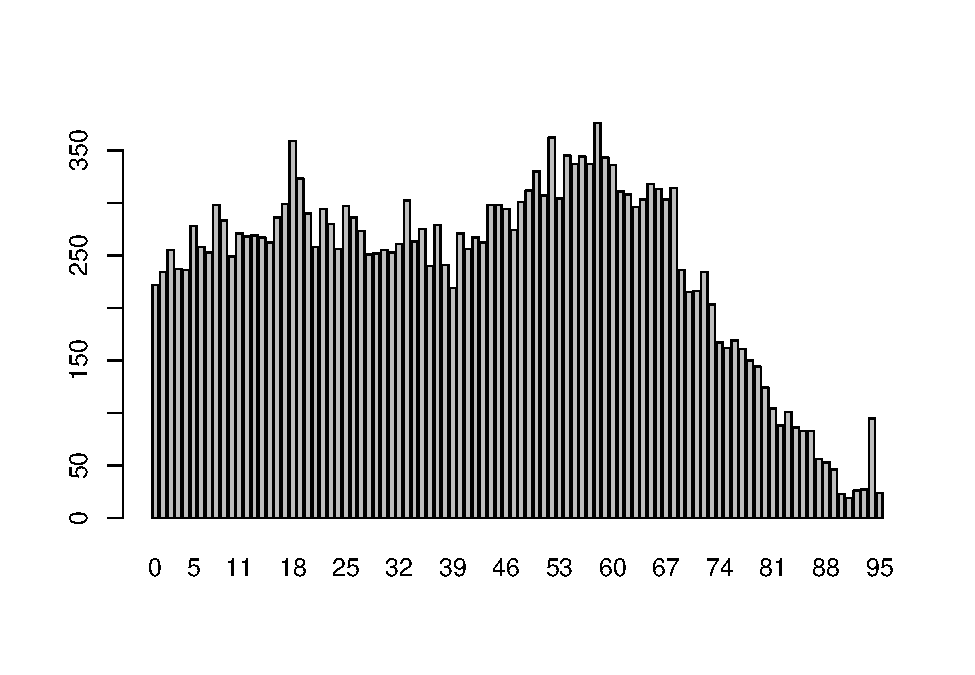
\includegraphics{_main_files/figure-latex/unnamed-chunk-17-1.pdf}

\hypertarget{glossary-1}{%
\section*{Glossary}\label{glossary-1}}
\addcontentsline{toc}{section}{Glossary}

\hypertarget{comparing-data}{%
\chapter{Comparing Data}\label{comparing-data}}

\textbf{NEEDS A LOT OF WORK}

\hypertarget{data-distributions}{%
\section{Data Distributions}\label{data-distributions}}

\hypertarget{normal-distributions}{%
\subsection{Normal Distributions}\label{normal-distributions}}

First we'll generate a normal distribution with the \texttt{rnorm()} function. This takes 3 arguments: \texttt{n,\ mean,\ sd}, which you can see filled in below. While we could print out a list of all these values, it's not easy to \emph{understand} a list of numbers

\begin{Shaded}
\begin{Highlighting}[]
\NormalTok{normal\_dist }\OtherTok{\textless{}{-}} \FunctionTok{rnorm}\NormalTok{(}\AttributeTok{n =} \DecValTok{100}\NormalTok{, }\DocumentationTok{\#\# 100 samples}
                     \AttributeTok{mean =} \DecValTok{10}\NormalTok{, }\DocumentationTok{\#\# with a mean of 10}
                     \AttributeTok{sd =} \DecValTok{1} \DocumentationTok{\#\# and a standard deviation of 1}
\NormalTok{                     )}


\NormalTok{normal\_dist}
\end{Highlighting}
\end{Shaded}

\begin{verbatim}
##   [1] 11.461743  9.228759 10.344360  9.011577 10.213482 10.412601  9.794298
##   [8] 10.493866  9.504083 11.064996  9.699334  9.528765  9.695063 10.451686
##  [15] 10.087802 11.458674  9.130766 11.169342 10.501660 10.984828 11.153812
##  [22]  9.105005  8.527781  9.019875 10.992873  9.472671  9.630453 11.930379
##  [29]  9.709972  8.915032  9.977849  9.884639 11.264260  8.107857 10.610282
##  [36]  9.271024 11.340466  9.056360  9.240962 10.841711  9.398378 10.762601
##  [43] 10.920869 10.909921 12.515859  9.062207 10.473640  9.640756 10.307330
##  [50]  9.751568  9.465202  9.822931 10.427316  8.177950 10.831855  9.578186
##  [57]  9.241150 11.090053 10.497670  8.966486  8.757531  8.188186 10.269957
##  [64] 12.410783  9.922728 11.798599  9.000495  9.854824  9.246429 11.089729
##  [71] 10.751389 10.548314 11.734746  9.533314  9.581124 10.169512 10.257509
##  [78]  9.636182  8.602800 10.572997  9.692793  9.875417 11.153376 10.208966
##  [85] 11.528380 10.993645  9.387126 10.528465 11.308611 10.159791 10.715990
##  [92] 11.469583  9.847889  9.435087  9.826541 10.593494 11.558613 11.376639
##  [99] 10.062645 10.289308
\end{verbatim}

Another better way to look at data would be to \textbf{visualize} or \textbf{plot} it. One way to to that is with a \textbf{histogram}, which groups \textbf{continuous values} into \textbf{bins}, then plots the \textbf{frequency} for each bin.

In R, we use the \texttt{hist()} function to plot a histogram of data. We can (try to) control the number of bins with the \texttt{breaks} argument, but note that it doesn't always match up. The \texttt{hist()} function will adjust based on the distribution of the data.

\begin{Shaded}
\begin{Highlighting}[]
\FunctionTok{hist}\NormalTok{(normal\_dist,}\AttributeTok{breaks =} \DecValTok{5}\NormalTok{)}
\end{Highlighting}
\end{Shaded}

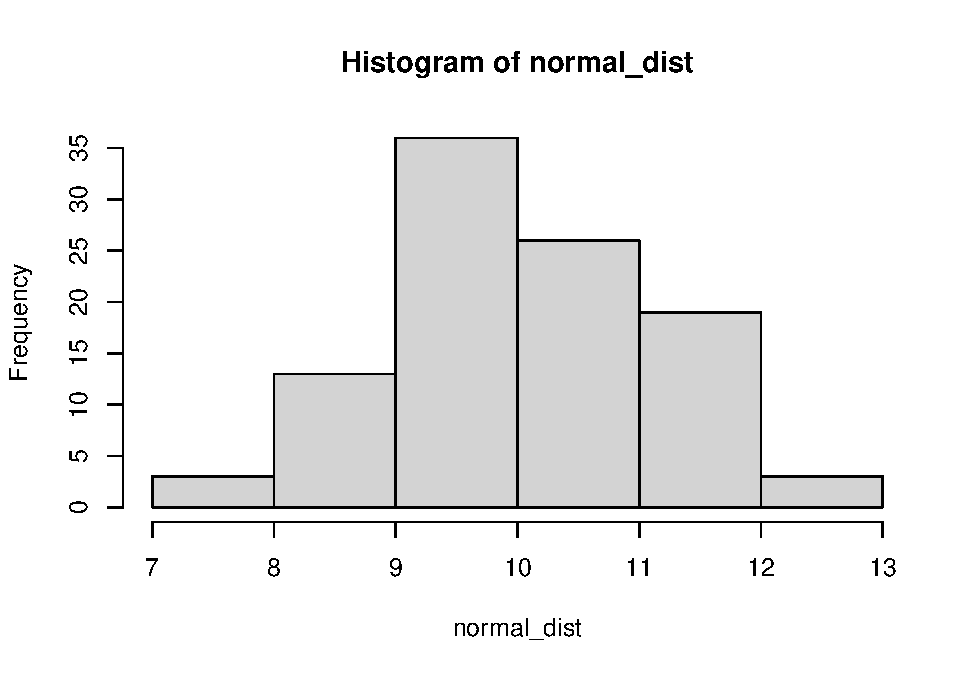
\includegraphics{_main_files/figure-latex/norm_dist_plot-1.pdf}

Another way to visualize this would be with a d

\hypertarget{what-is-normal}{%
\subsection{\texorpdfstring{What \emph{is} normal?}{What is normal?}}\label{what-is-normal}}

\hypertarget{quantitative-summaries}{%
\subsubsection{Quantitative summaries}\label{quantitative-summaries}}

5num summary
* Min, 25th percentile, median, 75th percentile, Max

\begin{Shaded}
\begin{Highlighting}[]
\NormalTok{tab\_normal\_dist }\OtherTok{\textless{}{-}} \FunctionTok{summary}\NormalTok{(normal\_dist)}
\end{Highlighting}
\end{Shaded}

We can print the table in R by calling its name.

\begin{Shaded}
\begin{Highlighting}[]
\NormalTok{tab\_normal\_dist}
\end{Highlighting}
\end{Shaded}

\begin{verbatim}
##    Min. 1st Qu.  Median    Mean 3rd Qu.    Max. 
##   8.108   9.496  10.165  10.161  10.859  12.516
\end{verbatim}

Mean, standard deviation

\hypertarget{meaningful-comparisons}{%
\subsubsection{Meaningful Comparisons}\label{meaningful-comparisons}}

How to compare apples to oranges? Standardize the units / standardize the data

\begin{Shaded}
\begin{Highlighting}[]
\NormalTok{data1 }\OtherTok{\textless{}{-}} \FunctionTok{rnorm}\NormalTok{(}\AttributeTok{n=}\DecValTok{1000}\NormalTok{, }
              \AttributeTok{mean =} \DecValTok{100}\NormalTok{,}
              \AttributeTok{sd =} \DecValTok{10}\NormalTok{)}

\NormalTok{data2 }\OtherTok{\textless{}{-}} \FunctionTok{rnorm}\NormalTok{(}\AttributeTok{n=}\DecValTok{1000}\NormalTok{,}
               \AttributeTok{mean =} \DecValTok{60}\NormalTok{, }
               \AttributeTok{sd =} \DecValTok{25}\NormalTok{)}
\end{Highlighting}
\end{Shaded}

Are these the same distribution?

Any issues??

\begin{Shaded}
\begin{Highlighting}[]
\FunctionTok{layout}\NormalTok{(}\FunctionTok{matrix}\NormalTok{(}\DecValTok{1}\SpecialCharTok{:}\DecValTok{2}\NormalTok{, }\AttributeTok{ncol =} \DecValTok{2}\NormalTok{))}
\FunctionTok{hist}\NormalTok{(data1)}
\FunctionTok{hist}\NormalTok{(data2)}
\end{Highlighting}
\end{Shaded}

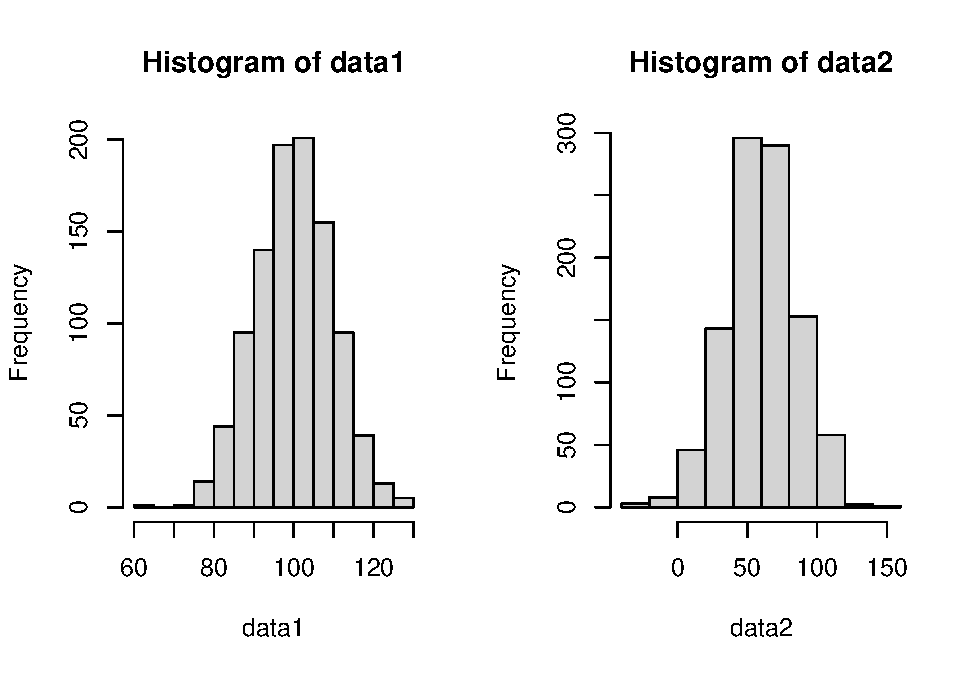
\includegraphics{_main_files/figure-latex/rnorm_hist_comp-1.pdf}

\begin{Shaded}
\begin{Highlighting}[]
\NormalTok{total\_range }\OtherTok{\textless{}{-}} \FunctionTok{range}\NormalTok{(data1, data2)}
\end{Highlighting}
\end{Shaded}

Are they the same?

\begin{Shaded}
\begin{Highlighting}[]
\FunctionTok{layout}\NormalTok{(}\FunctionTok{matrix}\NormalTok{(}\DecValTok{1}\SpecialCharTok{:}\DecValTok{2}\NormalTok{, }\AttributeTok{ncol =} \DecValTok{2}\NormalTok{))}
\FunctionTok{hist}\NormalTok{(data1, }\AttributeTok{xlim =}\NormalTok{ total\_range)}
\FunctionTok{hist}\NormalTok{(data2, }\AttributeTok{xlim =}\NormalTok{ total\_range)}
\end{Highlighting}
\end{Shaded}

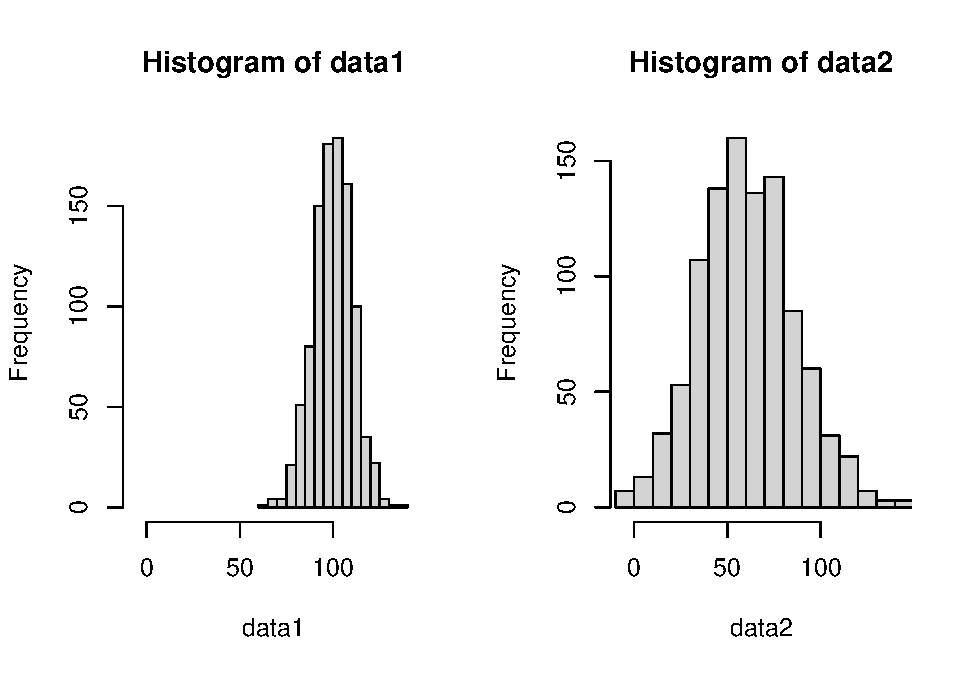
\includegraphics{_main_files/figure-latex/rnorm_hist_comp_true-1.pdf}

Numerically / tabularly

Often times its important to tables of \textbf{summary statistics}

\begin{Shaded}
\begin{Highlighting}[]
\NormalTok{norm\_comp\_tab }\OtherTok{\textless{}{-}} \FunctionTok{rbind}\NormalTok{(}\FunctionTok{summary}\NormalTok{(data1),}
                       \FunctionTok{summary}\NormalTok{(data2))}

\NormalTok{norm\_comp\_tab}
\end{Highlighting}
\end{Shaded}

\begin{verbatim}
##           Min.  1st Qu.    Median     Mean   3rd Qu.     Max.
## [1,]  61.97265 93.25935 100.31955 99.83822 106.85430 133.9527
## [2,] -34.25198 42.98023  59.75894 59.52261  76.50663 150.4806
\end{verbatim}

Making the table a little nicer. Also an example of \textbf{conditional programming}.

\begin{Shaded}
\begin{Highlighting}[]
\FunctionTok{rownames}\NormalTok{(norm\_comp\_tab) }\DocumentationTok{\#\# they\textquotesingle{}re null}
\end{Highlighting}
\end{Shaded}

\begin{verbatim}
## NULL
\end{verbatim}

\begin{Shaded}
\begin{Highlighting}[]
\ControlFlowTok{if}\NormalTok{(}\FunctionTok{is.null}\NormalTok{(}\FunctionTok{rownames}\NormalTok{(norm\_comp\_tab)))\{}
  \FunctionTok{rownames}\NormalTok{(norm\_comp\_tab) }\OtherTok{\textless{}{-}} \FunctionTok{c}\NormalTok{(}\StringTok{"data1"}\NormalTok{, }\StringTok{"data2"}\NormalTok{)}
\NormalTok{\}}
\end{Highlighting}
\end{Shaded}

When working with \textbf{Rmarkdown} we can take advantage of \texttt{knitr} and \texttt{pandoc} to nice looking tables even easier.

\begin{Shaded}
\begin{Highlighting}[]
\NormalTok{knitr}\SpecialCharTok{::}\FunctionTok{kable}\NormalTok{(norm\_comp\_tab)}
\end{Highlighting}
\end{Shaded}

\begin{tabular}{l|r|r|r|r|r|r}
\hline
  & Min. & 1st Qu. & Median & Mean & 3rd Qu. & Max.\\
\hline
data1 & 61.97265 & 93.25935 & 100.31955 & 99.83822 & 106.85430 & 133.9527\\
\hline
data2 & -34.25198 & 42.98023 & 59.75894 & 59.52261 & 76.50663 & 150.4806\\
\hline
\end{tabular}

\textbf{How} transform the data

Simple transformation (multiply all values by 100)
* to convert units
* other examples?

Complex transformations
* log-transformation (\emph{DEE: not a fan})
* z-scores (\emph{DEE: a better option})

\textbf{Why} transform the data?
* Real world applications?
* Is it always appropriate to transform data?

\hypertarget{skews}{%
\subsection{Skews}\label{skews}}

What to do if the data are \textbf{not} normal?

\hypertarget{statisitcal-testing-of-simple-data-sets}{%
\section{Statisitcal testing of simple data sets}\label{statisitcal-testing-of-simple-data-sets}}

\hypertarget{t-tests-anova-chi2}{%
\subsection{t-tests, ANOVA, chi2}\label{t-tests-anova-chi2}}

\hypertarget{relationships-between-variables-in-simple-data-sets}{%
\section{Relationships between variables in simple data sets}\label{relationships-between-variables-in-simple-data-sets}}

\hypertarget{correlation-linear-regression}{%
\subsection{Correlation, Linear Regression}\label{correlation-linear-regression}}

\hypertarget{simple-lm}{%
\subsubsection{Simple LM}\label{simple-lm}}

\hypertarget{complex-lm}{%
\subsubsection{Complex LM}\label{complex-lm}}

\hypertarget{genearlized-linear-model}{%
\subsection{Genearlized Linear Model}\label{genearlized-linear-model}}

For now, I have 3 main chapters for each of the main sections:
* Basics of data science / R \ref{unit1}
* Applications/critiques using IPUMS data \ref{unit2}
* Student-driven projects \ref{unit3}

Each of these \textbf{Chapters} contains multiple sections. We'll likely want to break these sections out into their own \texttt{.Rmd} files as they get fleshed out. For now, I'll try to keep the abundance of files limited.

\textbf{NOTE:} As these actually get filled out, we will probably want to insert different \texttt{part}s to the book (EG, the content of Unit 1 is covered in \texttt{Part\ I}).
* Declare parts with \texttt{\#\ (PART)\ Part\ I\ \{-\}} immediately before the first chapter \texttt{\#} it contains.

\textbf{Topics to include:}
* What is data?
* Everything can be data
* How do we interpret data
* Tables
* Plots
* Univariate distributions
* What can they tell us
* Multi-modality in distributions
* Categorical vs continuous data
* Don't need to get ahead of this yet
* Add in a grouping category - multi state/multi-national dataset
* Ttest / anova

\textbf{Type of Data:}
Age distributions
Specifically generate a dataset with old/young folks over-represented to highlight a bimodal distribution

Start with single state/country
Add a second state/country to demo ttest
Add more to demo anova

Alternatively, income by education level - may be more interesting/relevant to college students (or depressing)

\hypertarget{intro-to-rrstudio}{%
\section{Intro to R/RStudio}\label{intro-to-rrstudio}}

\hypertarget{reading-data-distributions}{%
\section{Reading Data / Distributions}\label{reading-data-distributions}}

\hypertarget{what-is-a-normal-distribution}{%
\subsection{\texorpdfstring{What \emph{is} a \textbf{normal distribution}}{What is a normal distribution}}\label{what-is-a-normal-distribution}}

\hypertarget{how-normal-is-it}{%
\subsubsection{How normal is it?}\label{how-normal-is-it}}

show increasingly unclear examples of normal vs not

introduce tests of normality

\hypertarget{measuring-normality---single-sample}{%
\subsubsection{Measuring normality - single sample}\label{measuring-normality---single-sample}}

reinforce {[}concept of statistical{]} \textbf{normality}

is a value from a sample? - one way ttest
something about tails

\hypertarget{comparing-normality---two-saples}{%
\subsubsection{comparing normality - two saples}\label{comparing-normality---two-saples}}

standard / two-way t test

\hypertarget{comparing-more-than-two---anova}{%
\subsubsection{comparing more than two - ANOVA}\label{comparing-more-than-two---anova}}

\hypertarget{glossary-2}{%
\section*{Glossary}\label{glossary-2}}
\addcontentsline{toc}{section}{Glossary}

Data
Quantitative
Qualitative
Discrete
Continuous
Nominal
Ordinal

\hypertarget{unit-2-ipums}{%
\chapter*{Unit 2: IPUMS}\label{unit-2-ipums}}
\addcontentsline{toc}{chapter}{Unit 2: IPUMS}

\hypertarget{lesson-6-introduction-to-ipums}{%
\section*{Lesson 6 Introduction to IPUMS}\label{lesson-6-introduction-to-ipums}}

Some text to break up the sub-section headers

\hypertarget{intro-to-ipums-website}{%
\subsection*{Intro to IPUMS website}\label{intro-to-ipums-website}}
\addcontentsline{toc}{subsection}{Intro to IPUMS website}

\hypertarget{background-on-ipums}{%
\subsection*{background on ipums}\label{background-on-ipums}}
\addcontentsline{toc}{subsection}{background on ipums}

\hypertarget{navigating-website}{%
\subsection*{navigating website}\label{navigating-website}}
\addcontentsline{toc}{subsection}{navigating website}

Find certain (very common) variables to answer (common) social science questions.

\hypertarget{lesson-7-exploratory-analysis}{%
\section*{Lesson 7 Exploratory analysis}\label{lesson-7-exploratory-analysis}}

If you've just collected a survey, or other raw data, you may not know what you're looking for. This is perfectly ok but goes against \emph{the scientific method} most people learned in grade school (More on that to follow(\textbf{\emph{include\_link}})).

This unit begins by presenting data/distributions and asking students to begin interpreting the data . visual exploration is encouraged and basic of data manipulation are taught
* \emph{EG:} how to subset data, how to reshape data, how to recode data, how to convert from one \texttt{data\ type} to another.

Example lab exercise:

Students given a data set (xls, csv, etc)
* load data, perform manipulations, basic summaries
+ cross tabs
+ group means by a covariate
* inspect data visually
+ \emph{DESCRIBE} the distribution - is it normal? significant?
* \emph{FIND} aquestion in the spread of the data
+ how can you test this (maybe small group work)
* write up/ present results
+ think on confounding factors / biases

\hypertarget{advanced-exploration---change-over-time}{%
\subsection*{Advanced Exploration - Change Over Time}\label{advanced-exploration---change-over-time}}
\addcontentsline{toc}{subsection}{Advanced Exploration - Change Over Time}

Here we demonstrate an approach to looking at how Family Structure (inferred from household relationships) has changed over time.

\hypertarget{setup-load-data}{%
\subsubsection*{Setup / Load Data}\label{setup-load-data}}
\addcontentsline{toc}{subsubsection}{Setup / Load Data}

Install/update R packages

\begin{Shaded}
\begin{Highlighting}[]
\FunctionTok{install.packages}\NormalTok{(}\StringTok{"ipumsr"}\NormalTok{)}
\FunctionTok{install.packages}\NormalTok{(}\StringTok{"tidyverse"}\NormalTok{)}
\end{Highlighting}
\end{Shaded}

Data extract created online using the datacart system.

\begin{Shaded}
\begin{Highlighting}[]
\FunctionTok{library}\NormalTok{(ipumsr)}
\FunctionTok{library}\NormalTok{(dplyr)}


\NormalTok{ddi }\OtherTok{\textless{}{-}} \FunctionTok{read\_ipums\_ddi}\NormalTok{(}\StringTok{"Data/ipumsi\_00005.xml"}\NormalTok{)}
\NormalTok{data }\OtherTok{\textless{}{-}} \FunctionTok{read\_ipums\_micro}\NormalTok{(ddi)}
\end{Highlighting}
\end{Shaded}

\hypertarget{inspect-the-data-1}{%
\paragraph*{Inspect the Data}\label{inspect-the-data-1}}
\addcontentsline{toc}{paragraph}{Inspect the Data}

Using \texttt{haven} labeled values.

\begin{Shaded}
\begin{Highlighting}[]
\NormalTok{data}\SpecialCharTok{$}\NormalTok{RELATE[}\DecValTok{1}\SpecialCharTok{:}\DecValTok{100}\NormalTok{]}
\FunctionTok{class}\NormalTok{(data}\SpecialCharTok{$}\NormalTok{RELATE)}

\NormalTok{data }\SpecialCharTok{\%\textgreater{}\%} \FunctionTok{count}\NormalTok{(RELATE)}
\NormalTok{data }\SpecialCharTok{\%\textgreater{}\%} \FunctionTok{count}\NormalTok{(SEX)}
\end{Highlighting}
\end{Shaded}

What were those codes ??

\begin{Shaded}
\begin{Highlighting}[]
\DocumentationTok{\#\# need to convert this to an image or something similar; kable table?}
\FunctionTok{ipums\_view}\NormalTok{(ddi)}
\end{Highlighting}
\end{Shaded}

\hypertarget{visualize}{%
\paragraph*{Visualize}\label{visualize}}
\addcontentsline{toc}{paragraph}{Visualize}

A simple plot

\begin{Shaded}
\begin{Highlighting}[]
\FunctionTok{plot}\NormalTok{(AGE }\SpecialCharTok{\textasciitilde{}}\NormalTok{ YEAR, }\AttributeTok{data =}\NormalTok{ data)}
\end{Highlighting}
\end{Shaded}

A fancier plot

\begin{Shaded}
\begin{Highlighting}[]
\FunctionTok{plot}\NormalTok{(AGE}\SpecialCharTok{\textasciitilde{}}\NormalTok{YEAR, }\AttributeTok{data =}\NormalTok{ data, }\AttributeTok{type =} \StringTok{"n"}\NormalTok{, }\AttributeTok{main =} \StringTok{"Age by Sex, over Time, CO"}\NormalTok{)}
\FunctionTok{points}\NormalTok{(data}\SpecialCharTok{$}\NormalTok{YEAR[data}\SpecialCharTok{$}\NormalTok{SEX}\SpecialCharTok{==}\DecValTok{1}\NormalTok{]}\SpecialCharTok{{-}}\DecValTok{1}\NormalTok{, data}\SpecialCharTok{$}\NormalTok{AGE[data}\SpecialCharTok{$}\NormalTok{SEX}\SpecialCharTok{==}\DecValTok{1}\NormalTok{], }\AttributeTok{pch =} \DecValTok{16}\NormalTok{, }\AttributeTok{col =} \FunctionTok{hsv}\NormalTok{(.}\DecValTok{6}\NormalTok{,.}\DecValTok{6}\NormalTok{,.}\DecValTok{8}\NormalTok{,.}\DecValTok{2}\NormalTok{))}

\FunctionTok{points}\NormalTok{(data}\SpecialCharTok{$}\NormalTok{YEAR[data}\SpecialCharTok{$}\NormalTok{SEX}\SpecialCharTok{==}\DecValTok{2}\NormalTok{]}\SpecialCharTok{+}\DecValTok{1}\NormalTok{, data}\SpecialCharTok{$}\NormalTok{AGE[data}\SpecialCharTok{$}\NormalTok{SEX}\SpecialCharTok{==}\DecValTok{2}\NormalTok{], }\AttributeTok{pch =} \DecValTok{16}\NormalTok{, }\AttributeTok{col =} \FunctionTok{hsv}\NormalTok{(}\DecValTok{1}\NormalTok{,.}\DecValTok{6}\NormalTok{,.}\DecValTok{8}\NormalTok{,.}\DecValTok{2}\NormalTok{))}

\FunctionTok{abline}\NormalTok{(}\FunctionTok{lm}\NormalTok{(AGE}\SpecialCharTok{\textasciitilde{}}\NormalTok{YEAR, }\AttributeTok{data =}\NormalTok{ data), }\AttributeTok{col =} \StringTok{"green"}\NormalTok{)}
\end{Highlighting}
\end{Shaded}

\hypertarget{asking-logical-questions}{%
\paragraph*{Asking (logical) questions}\label{asking-logical-questions}}
\addcontentsline{toc}{paragraph}{Asking (logical) questions}

Here we demonstrate how setting up logical questions can be used to easily filter/subset data.

\begin{Shaded}
\begin{Highlighting}[]
\NormalTok{age\_test }\OtherTok{\textless{}{-}}\NormalTok{ data}\SpecialCharTok{$}\NormalTok{AGE }\SpecialCharTok{\textgreater{}} \DecValTok{18}

\FunctionTok{class}\NormalTok{(age\_test)}

\NormalTok{age\_test}
\end{Highlighting}
\end{Shaded}

Logical vectors are stored as \texttt{TRUE} or \texttt{FALSE}, but can also be evaluated numerically as \texttt{1} or \texttt{0} respectively. We can therefore \texttt{sum()} the number of \texttt{TRUE} values and divide by total rows for a proportion.

\begin{Shaded}
\begin{Highlighting}[]
\FunctionTok{sum}\NormalTok{(age\_test)}\SpecialCharTok{/}\FunctionTok{nrow}\NormalTok{(data)}
\end{Highlighting}
\end{Shaded}

\hypertarget{hh-vs-persons}{%
\paragraph*{HH vs persons}\label{hh-vs-persons}}
\addcontentsline{toc}{paragraph}{HH vs persons}

A unique characteristic of census and some survey data is the nested-structure with individuals being grouped into households. Often times it is necessary to choose to work at the hh or person level, and data must be appropriately manipulated to fit that case.

\begin{Shaded}
\begin{Highlighting}[]
\NormalTok{hh\_total }\OtherTok{\textless{}{-}} \FunctionTok{length}\NormalTok{(}\FunctionTok{unique}\NormalTok{(data}\SpecialCharTok{$}\NormalTok{SERIAL))}
\NormalTok{hh\_total}
\FunctionTok{ipums\_view}\NormalTok{(ddi)}
\end{Highlighting}
\end{Shaded}

\hypertarget{nuclear-family}{%
\subsubsection*{Nuclear Family}\label{nuclear-family}}
\addcontentsline{toc}{subsubsection}{Nuclear Family}

First we look at a nuclear family, comprising only parents and their immediate children.

\begin{Shaded}
\begin{Highlighting}[]
\FunctionTok{library}\NormalTok{(ipumsr)}
\FunctionTok{library}\NormalTok{(dplyr)}

\NormalTok{ddi }\OtherTok{\textless{}{-}} \FunctionTok{read\_ipums\_ddi}\NormalTok{(}\StringTok{"/pkg/ipums/personal/ehrli097/AABA\_2022/Data/ipumsi\_00005.xml"}\NormalTok{)}
\NormalTok{all\_data }\OtherTok{\textless{}{-}} \FunctionTok{read\_ipums\_micro}\NormalTok{(ddi)}

\NormalTok{census\_years }\OtherTok{\textless{}{-}} \FunctionTok{c}\NormalTok{(}\DecValTok{1860}\NormalTok{, }\DecValTok{1870}\NormalTok{, }\DecValTok{1880}\NormalTok{, }\DecValTok{1900}\NormalTok{, }\DecValTok{1910}\NormalTok{, }\DecValTok{1960}\NormalTok{, }\DecValTok{1970}\NormalTok{, }\DecValTok{1980}\NormalTok{, }\DecValTok{1990}\NormalTok{, }\DecValTok{2000}\NormalTok{, }\DecValTok{2010}\NormalTok{)}

\DocumentationTok{\#\# subset census only}
\NormalTok{d2 }\OtherTok{\textless{}{-}}\NormalTok{ all\_data }\SpecialCharTok{\%\textgreater{}\%} \FunctionTok{filter}\NormalTok{(YEAR }\SpecialCharTok{\%in\%}\NormalTok{ census\_years)}

\DocumentationTok{\#\# make a household dataframe}
\NormalTok{hhs }\OtherTok{\textless{}{-}}\NormalTok{ d2 }\SpecialCharTok{\%\textgreater{}\%} \FunctionTok{distinct}\NormalTok{(YEAR, SERIAL, }\AttributeTok{.keep\_all =} \ConstantTok{TRUE}\NormalTok{) }\SpecialCharTok{\%\textgreater{}\%} \FunctionTok{select}\NormalTok{(YEAR,SERIAL,GEO1\_US)}

\NormalTok{hhs }\SpecialCharTok{\%\textgreater{}\%} \FunctionTok{View}\NormalTok{()}
\end{Highlighting}
\end{Shaded}

\begin{Shaded}
\begin{Highlighting}[]
\NormalTok{hhs }\OtherTok{\textless{}{-}}\NormalTok{ d2 }\SpecialCharTok{\%\textgreater{}\%} \FunctionTok{filter}\NormalTok{(RELATE }\SpecialCharTok{==}\DecValTok{4}\NormalTok{) }\SpecialCharTok{\%\textgreater{}\%} 
  
  
  \FunctionTok{distinct}\NormalTok{(YEAR, SERIAL) }\SpecialCharTok{\%\textgreater{}\%} \FunctionTok{mutate}\NormalTok{(}\AttributeTok{extended\_test=}\ConstantTok{TRUE}\NormalTok{) }\SpecialCharTok{\%\textgreater{}\%} \FunctionTok{right\_join}\NormalTok{(hhs, }\AttributeTok{by =} \FunctionTok{c}\NormalTok{(}\StringTok{"YEAR"}\NormalTok{, }\StringTok{"SERIAL"}\NormalTok{)) }\SpecialCharTok{\%\textgreater{}\%} \FunctionTok{mutate}\NormalTok{(}\AttributeTok{extended\_test=}\FunctionTok{if\_else}\NormalTok{(}\FunctionTok{is.na}\NormalTok{(extended\_test),}\ConstantTok{FALSE}\NormalTok{,}\ConstantTok{TRUE}\NormalTok{))}
  








\NormalTok{hhs }\OtherTok{\textless{}{-}}\NormalTok{ d2 }\SpecialCharTok{\%\textgreater{}\%} \FunctionTok{filter}\NormalTok{(}\SpecialCharTok{!}\NormalTok{RELATE }\SpecialCharTok{\%in\%} \FunctionTok{c}\NormalTok{(}\DecValTok{1}\NormalTok{, }\DecValTok{2}\NormalTok{, }\DecValTok{3}\NormalTok{) }\SpecialCharTok{|}
\NormalTok{                  (RELATE }\SpecialCharTok{==} \DecValTok{3} \SpecialCharTok{\&}
\NormalTok{                     MARST }\SpecialCharTok{\%in\%} \FunctionTok{c}\NormalTok{(}\DecValTok{2}\NormalTok{, }\DecValTok{3}\NormalTok{, }\DecValTok{4}\NormalTok{))}
\NormalTok{                ) }\SpecialCharTok{\%\textgreater{}\%} 

  
  
  \FunctionTok{distinct}\NormalTok{(YEAR, SERIAL) }\SpecialCharTok{\%\textgreater{}\%} \FunctionTok{mutate}\NormalTok{(}\AttributeTok{nuclear\_test =} \ConstantTok{FALSE}\NormalTok{) }\SpecialCharTok{\%\textgreater{}\%} \FunctionTok{right\_join}\NormalTok{(hhs, }\AttributeTok{by =} \FunctionTok{c}\NormalTok{(}\StringTok{"YEAR"}\NormalTok{, }\StringTok{"SERIAL"}\NormalTok{)) }\SpecialCharTok{\%\textgreater{}\%} \FunctionTok{mutate}\NormalTok{(}\AttributeTok{nuclear\_test =} \FunctionTok{if\_else}\NormalTok{(}\FunctionTok{is.na}\NormalTok{(nuclear\_test), }\ConstantTok{TRUE}\NormalTok{, }\ConstantTok{FALSE}\NormalTok{))}



\FunctionTok{table}\NormalTok{(hhs}\SpecialCharTok{$}\NormalTok{extended\_test,hhs}\SpecialCharTok{$}\NormalTok{nuclear\_test)}
\end{Highlighting}
\end{Shaded}

\hypertarget{tabulate-results}{%
\paragraph*{Tabulate results}\label{tabulate-results}}
\addcontentsline{toc}{paragraph}{Tabulate results}

\begin{Shaded}
\begin{Highlighting}[]
\NormalTok{  hhs }\OtherTok{\textless{}{-}}\NormalTok{ d2 }\SpecialCharTok{\%\textgreater{}\%} \FunctionTok{filter}\NormalTok{(RELATED }\SpecialCharTok{\%in\%} \FunctionTok{c}\NormalTok{(}\DecValTok{4200}\NormalTok{, }\DecValTok{4210}\NormalTok{, }\DecValTok{4211}\NormalTok{, }\DecValTok{4220}\NormalTok{, }\DecValTok{4500}\NormalTok{, }\DecValTok{4510}\NormalTok{, }\DecValTok{4600}\NormalTok{)) }\SpecialCharTok{\%\textgreater{}\%} \FunctionTok{distinct}\NormalTok{(YEAR, SERIAL) }\SpecialCharTok{\%\textgreater{}\%} \FunctionTok{mutate}\NormalTok{(}\AttributeTok{parent\_test=}\ConstantTok{TRUE}\NormalTok{) }\SpecialCharTok{\%\textgreater{}\%} \FunctionTok{right\_join}\NormalTok{(hhs, }\AttributeTok{by =} \FunctionTok{c}\NormalTok{(}\StringTok{"YEAR"}\NormalTok{, }\StringTok{"SERIAL"}\NormalTok{)) }\SpecialCharTok{\%\textgreater{}\%} \FunctionTok{mutate}\NormalTok{(}\AttributeTok{parent\_test=}\FunctionTok{if\_else}\NormalTok{(}\FunctionTok{is.na}\NormalTok{(parent\_test),}\ConstantTok{FALSE}\NormalTok{,}\ConstantTok{TRUE}\NormalTok{))}


\NormalTok{  hhs }\OtherTok{\textless{}{-}}\NormalTok{ d2 }\SpecialCharTok{\%\textgreater{}\%} \FunctionTok{filter}\NormalTok{(RELATED }\SpecialCharTok{\%in\%} \FunctionTok{c}\NormalTok{(}\DecValTok{4100}\NormalTok{, }\DecValTok{4110}\NormalTok{, }\DecValTok{4120}\NormalTok{, }\DecValTok{4130}\NormalTok{, }\DecValTok{4300}\NormalTok{, }\DecValTok{4301}\NormalTok{, }\DecValTok{4302}\NormalTok{)) }\SpecialCharTok{\%\textgreater{}\%} \FunctionTok{distinct}\NormalTok{(YEAR, SERIAL) }\SpecialCharTok{\%\textgreater{}\%} \FunctionTok{mutate}\NormalTok{(}\AttributeTok{children\_test=}\ConstantTok{TRUE}\NormalTok{) }\SpecialCharTok{\%\textgreater{}\%} \FunctionTok{right\_join}\NormalTok{(hhs, }\AttributeTok{by =} \FunctionTok{c}\NormalTok{(}\StringTok{"YEAR"}\NormalTok{, }\StringTok{"SERIAL"}\NormalTok{)) }\SpecialCharTok{\%\textgreater{}\%} \FunctionTok{mutate}\NormalTok{(}\AttributeTok{children\_test=}\FunctionTok{if\_else}\NormalTok{(}\FunctionTok{is.na}\NormalTok{(children\_test),}\ConstantTok{FALSE}\NormalTok{,}\ConstantTok{TRUE}\NormalTok{))}
  
  
\NormalTok{  res\_tabs }\OtherTok{\textless{}{-}} \FunctionTok{list}\NormalTok{(}
    \StringTok{"nuclear\_test"} \OtherTok{=}\NormalTok{ hhs }\SpecialCharTok{\%\textgreater{}\%} \FunctionTok{group\_by}\NormalTok{(YEAR, nuclear\_test,GEO1\_US) }\SpecialCharTok{\%\textgreater{}\%} \FunctionTok{summarize}\NormalTok{(}\AttributeTok{.groups=}\StringTok{"drop"}\NormalTok{,}\AttributeTok{n =} \FunctionTok{n}\NormalTok{()) }\SpecialCharTok{\%\textgreater{}\%} \FunctionTok{as.data.frame}\NormalTok{(),}
  \StringTok{"extended\_test"} \OtherTok{=}\NormalTok{ hhs }\SpecialCharTok{\%\textgreater{}\%} \FunctionTok{group\_by}\NormalTok{(YEAR, extended\_test, GEO1\_US) }\SpecialCharTok{\%\textgreater{}\%} \FunctionTok{summarize}\NormalTok{(}\AttributeTok{.groups=}\StringTok{"drop"}\NormalTok{,}\AttributeTok{n =} \FunctionTok{n}\NormalTok{()) }\SpecialCharTok{\%\textgreater{}\%} \FunctionTok{as.data.frame}\NormalTok{(),}
  \StringTok{"parent\_test"} \OtherTok{=}\NormalTok{ hhs }\SpecialCharTok{\%\textgreater{}\%} \FunctionTok{group\_by}\NormalTok{(YEAR, parent\_test, GEO1\_US) }\SpecialCharTok{\%\textgreater{}\%} \FunctionTok{summarize}\NormalTok{(}\AttributeTok{.groups=}\StringTok{"drop"}\NormalTok{,}\AttributeTok{n =} \FunctionTok{n}\NormalTok{()) }\SpecialCharTok{\%\textgreater{}\%} \FunctionTok{as.data.frame}\NormalTok{(),}
  \StringTok{"children\_test"} \OtherTok{=}\NormalTok{ hhs }\SpecialCharTok{\%\textgreater{}\%} \FunctionTok{group\_by}\NormalTok{(YEAR, children\_test, GEO1\_US) }\SpecialCharTok{\%\textgreater{}\%} \FunctionTok{summarize}\NormalTok{(}\AttributeTok{.groups=}\StringTok{"drop"}\NormalTok{,}\AttributeTok{n =} \FunctionTok{n}\NormalTok{()) }\SpecialCharTok{\%\textgreater{}\%} \FunctionTok{as.data.frame}\NormalTok{()}
\NormalTok{  )}
  
  
  
  

\NormalTok{collapsed\_results }\OtherTok{\textless{}{-}}\NormalTok{ res\_tabs }\SpecialCharTok{\%\textgreater{}\%}\NormalTok{ purrr}\SpecialCharTok{::}\FunctionTok{map}\NormalTok{(}\ControlFlowTok{function}\NormalTok{(x)\{}
\NormalTok{  x }\OtherTok{\textless{}{-}}\NormalTok{ x }\SpecialCharTok{\%\textgreater{}\%} \FunctionTok{group\_by}\NormalTok{(}\FunctionTok{across}\NormalTok{(}\FunctionTok{names}\NormalTok{(x)[}\DecValTok{1}\SpecialCharTok{:}\DecValTok{3}\NormalTok{])) }\SpecialCharTok{\%\textgreater{}\%} \FunctionTok{summarize}\NormalTok{(}\AttributeTok{.groups=}\StringTok{"drop"}\NormalTok{,}\AttributeTok{n =} \FunctionTok{sum}\NormalTok{(n))}

\NormalTok{\})}


\NormalTok{collapsed\_results }\OtherTok{\textless{}{-}} \FunctionTok{lapply}\NormalTok{(collapsed\_results, }\ControlFlowTok{function}\NormalTok{(x)\{}
  \FunctionTok{colnames}\NormalTok{(x)[}\DecValTok{2}\NormalTok{] }\OtherTok{\textless{}{-}} \StringTok{"test"}
  \FunctionTok{colnames}\NormalTok{(x)[}\DecValTok{3}\NormalTok{] }\OtherTok{\textless{}{-}} \StringTok{"state"}
  \FunctionTok{return}\NormalTok{(x)}
\NormalTok{\})}

\NormalTok{combined }\OtherTok{\textless{}{-}}\NormalTok{ collapsed\_results }\SpecialCharTok{\%\textgreater{}\%}\NormalTok{ purrr}\SpecialCharTok{::}\FunctionTok{reduce}\NormalTok{(full\_join, }\AttributeTok{by =} \FunctionTok{c}\NormalTok{(}\StringTok{"YEAR"}\NormalTok{, }\StringTok{"test"}\NormalTok{, }\StringTok{"state"}\NormalTok{))}



\FunctionTok{colnames}\NormalTok{(combined) }\OtherTok{\textless{}{-}} \FunctionTok{c}\NormalTok{(}\StringTok{"YEAR"}\NormalTok{,}\StringTok{"test"}\NormalTok{, }\StringTok{"state"}\NormalTok{, }\StringTok{"n\_nuclear"}\NormalTok{, }\StringTok{"n\_extended"}\NormalTok{, }\StringTok{"n\_parent"}\NormalTok{, }\StringTok{"n\_children"}\NormalTok{)}

\NormalTok{combined[}\FunctionTok{is.na}\NormalTok{(combined)] }\OtherTok{\textless{}{-}} \DecValTok{0}


\NormalTok{to\_plot }\OtherTok{\textless{}{-}}\NormalTok{ combined }\SpecialCharTok{\%\textgreater{}\%} \FunctionTok{group\_by}\NormalTok{(YEAR, state) }\SpecialCharTok{\%\textgreater{}\%} \FunctionTok{mutate}\NormalTok{(}\AttributeTok{n\_tot =} \FunctionTok{sum}\NormalTok{(n\_nuclear)) }\SpecialCharTok{\%\textgreater{}\%} \FunctionTok{ungroup}\NormalTok{() }\SpecialCharTok{\%\textgreater{}\%} \FunctionTok{mutate}\NormalTok{(}\AttributeTok{pct =}  \FunctionTok{across}\NormalTok{(}\FunctionTok{starts\_with}\NormalTok{(}\StringTok{"n\_"}\NormalTok{))}\SpecialCharTok{/}\NormalTok{n\_tot) }\SpecialCharTok{\%\textgreater{}\%} \FunctionTok{select}\NormalTok{(YEAR,test,state,pct)}
\end{Highlighting}
\end{Shaded}

\hypertarget{visualize-nuclear-families}{%
\paragraph*{Visualize Nuclear Families}\label{visualize-nuclear-families}}
\addcontentsline{toc}{paragraph}{Visualize Nuclear Families}

\begin{Shaded}
\begin{Highlighting}[]
\NormalTok{to\_plot }\OtherTok{\textless{}{-}}\NormalTok{ to\_plot }\SpecialCharTok{\%\textgreater{}\%} \FunctionTok{filter}\NormalTok{(test}\SpecialCharTok{==}\ConstantTok{TRUE}\NormalTok{)}



\FunctionTok{plot}\NormalTok{(to\_plot}\SpecialCharTok{$}\NormalTok{YEAR, to\_plot}\SpecialCharTok{$}\NormalTok{pct}\SpecialCharTok{$}\NormalTok{n\_nuclear, }\AttributeTok{col =} \FunctionTok{hsv}\NormalTok{(.}\DecValTok{4}\NormalTok{, .}\DecValTok{6}\NormalTok{,.}\DecValTok{8}\NormalTok{), }\AttributeTok{pch =} \DecValTok{16}\NormalTok{, }\AttributeTok{ylim =}\FunctionTok{c}\NormalTok{(}\DecValTok{0}\NormalTok{,}\DecValTok{1}\NormalTok{), }\AttributeTok{xlab =} \StringTok{""}\NormalTok{, }\AttributeTok{ylab =} \StringTok{"prop of hhs"}\NormalTok{, }\AttributeTok{main =} \StringTok{"Nuclear HHs over time in CO"}\NormalTok{)}
\end{Highlighting}
\end{Shaded}

\hypertarget{extended-family}{%
\subsubsection*{Extended Family}\label{extended-family}}
\addcontentsline{toc}{subsubsection}{Extended Family}

Next we look at hhs with extended families present. IE, any that contain more relationships than just Parent/Child/Sibling (between children only)

\hypertarget{gernerate-models}{%
\paragraph*{Gernerate models}\label{gernerate-models}}
\addcontentsline{toc}{paragraph}{Gernerate models}

\begin{Shaded}
\begin{Highlighting}[]
\NormalTok{to\_plot }\OtherTok{\textless{}{-}}\NormalTok{ to\_plot }\SpecialCharTok{\%\textgreater{}\%} \FunctionTok{filter}\NormalTok{(test}\SpecialCharTok{==}\ConstantTok{TRUE}\NormalTok{)}


\NormalTok{glm\_hist }\OtherTok{\textless{}{-}} \FunctionTok{glm}\NormalTok{(pct}\SpecialCharTok{$}\NormalTok{n\_extended }\SpecialCharTok{\textasciitilde{}}\NormalTok{ YEAR, }\AttributeTok{data =}\NormalTok{ to\_plot[to\_plot}\SpecialCharTok{$}\NormalTok{YEAR }\SpecialCharTok{\textless{}} \DecValTok{1950}\NormalTok{,], }\AttributeTok{family =} \FunctionTok{quasibinomial}\NormalTok{(}\AttributeTok{link=}\NormalTok{logit))}



\NormalTok{glm\_hist\_x }\OtherTok{\textless{}{-}} \FunctionTok{seq}\NormalTok{(}\AttributeTok{from=}\DecValTok{1860}\NormalTok{, }\AttributeTok{to =} \DecValTok{1910}\NormalTok{, }\AttributeTok{length.out =} \DecValTok{100}\NormalTok{)}
\NormalTok{glm\_hist\_y }\OtherTok{\textless{}{-}} \FunctionTok{predict}\NormalTok{(glm\_hist, }\FunctionTok{list}\NormalTok{(}\AttributeTok{YEAR =}\NormalTok{ glm\_hist\_x), }\AttributeTok{type =} \StringTok{"response"}\NormalTok{)}

\NormalTok{glm\_mod }\OtherTok{\textless{}{-}} \FunctionTok{glm}\NormalTok{(pct}\SpecialCharTok{$}\NormalTok{n\_extended }\SpecialCharTok{\textasciitilde{}}\NormalTok{ YEAR, }\AttributeTok{data =}\NormalTok{ to\_plot[to\_plot}\SpecialCharTok{$}\NormalTok{YEAR}\SpecialCharTok{\textgreater{}} \DecValTok{1950}\NormalTok{,], }\AttributeTok{family =} \FunctionTok{quasibinomial}\NormalTok{(}\AttributeTok{link=}\NormalTok{logit))}

\NormalTok{glm\_mod\_x }\OtherTok{\textless{}{-}} \FunctionTok{seq}\NormalTok{(}\AttributeTok{from =} \DecValTok{1960}\NormalTok{, }\AttributeTok{to =} \DecValTok{2010}\NormalTok{, }\AttributeTok{length.out =} \DecValTok{100}\NormalTok{)}
\NormalTok{glm\_mod\_y }\OtherTok{\textless{}{-}} \FunctionTok{predict}\NormalTok{(glm\_mod, }\FunctionTok{list}\NormalTok{(}\AttributeTok{YEAR =}\NormalTok{ glm\_mod\_x), }\AttributeTok{type =} \StringTok{"response"}\NormalTok{)}

\NormalTok{mods }\OtherTok{\textless{}{-}} \FunctionTok{list}\NormalTok{(}\StringTok{"hist"}\OtherTok{=}\FunctionTok{list}\NormalTok{(),}
             \StringTok{"mod"} \OtherTok{=} \FunctionTok{list}\NormalTok{()}
\NormalTok{             )}
\NormalTok{mods\_plots }\OtherTok{\textless{}{-}} \FunctionTok{list}\NormalTok{(}\StringTok{"hist"}\OtherTok{=}\FunctionTok{list}\NormalTok{(),}
                   \StringTok{"mod"} \OtherTok{=}\FunctionTok{list}\NormalTok{()}
\NormalTok{                   )}

\ControlFlowTok{for}\NormalTok{(i }\ControlFlowTok{in} \FunctionTok{names}\NormalTok{(to\_plot}\SpecialCharTok{$}\NormalTok{pct))\{}
  
\NormalTok{  hist\_x }\OtherTok{\textless{}{-}}\NormalTok{ to\_plot}\SpecialCharTok{$}\NormalTok{YEAR[to\_plot}\SpecialCharTok{$}\NormalTok{YEAR }\SpecialCharTok{\textless{}} \DecValTok{1950}\NormalTok{]}
\NormalTok{mod\_x }\OtherTok{\textless{}{-}}\NormalTok{ to\_plot}\SpecialCharTok{$}\NormalTok{YEAR[to\_plot}\SpecialCharTok{$}\NormalTok{YEAR }\SpecialCharTok{\textgreater{}} \DecValTok{1950}\NormalTok{]}

\NormalTok{  mods}\SpecialCharTok{$}\NormalTok{hist[[i]] }\OtherTok{\textless{}{-}} \FunctionTok{lm}\NormalTok{(pct[[i]] }\SpecialCharTok{\textasciitilde{}}\NormalTok{ YEAR, }\AttributeTok{data =}\NormalTok{ to\_plot[to\_plot}\SpecialCharTok{$}\NormalTok{YEAR }\SpecialCharTok{\textless{}} \DecValTok{1950}\NormalTok{,])}
  
\NormalTok{  mods\_plots}\SpecialCharTok{$}\NormalTok{hist[[i]] }\OtherTok{\textless{}{-}} 
    \FunctionTok{data.frame}\NormalTok{(}\StringTok{"x"} \OtherTok{=}\NormalTok{ hist\_x,}
               \StringTok{"y"} \OtherTok{=} \FunctionTok{predict}\NormalTok{(mods}\SpecialCharTok{$}\NormalTok{hist[[i]], }
                             \FunctionTok{list}\NormalTok{(}\AttributeTok{YEAR =}\NormalTok{hist\_x), }
                             \AttributeTok{type =} \StringTok{"response"}\NormalTok{)}
\NormalTok{               )}
  
  
  
\NormalTok{  mods}\SpecialCharTok{$}\NormalTok{mod[[i]] }\OtherTok{\textless{}{-}} \FunctionTok{lm}\NormalTok{(pct[[i]] }\SpecialCharTok{\textasciitilde{}}\NormalTok{ YEAR, }\AttributeTok{data =}\NormalTok{ to\_plot[to\_plot}\SpecialCharTok{$}\NormalTok{YEAR }\SpecialCharTok{\textgreater{}} \DecValTok{1950}\NormalTok{,])}
  
  
\NormalTok{  mods\_plots}\SpecialCharTok{$}\NormalTok{mod[[i]] }\OtherTok{\textless{}{-}} 
    \FunctionTok{data.frame}\NormalTok{(}\StringTok{"x"} \OtherTok{=}\NormalTok{ mod\_x,}
               \StringTok{"y"} \OtherTok{=} \FunctionTok{predict}\NormalTok{(mods}\SpecialCharTok{$}\NormalTok{mod[[i]], }
                             \FunctionTok{list}\NormalTok{(}\AttributeTok{YEAR =}\NormalTok{mod\_x), }
                             \AttributeTok{type =} \StringTok{"response"}\NormalTok{)}
\NormalTok{               )}
\NormalTok{\}}
\end{Highlighting}
\end{Shaded}

\hypertarget{visualize-1}{%
\paragraph*{Visualize}\label{visualize-1}}
\addcontentsline{toc}{paragraph}{Visualize}

\begin{Shaded}
\begin{Highlighting}[]
\FunctionTok{plot}\NormalTok{(to\_plot}\SpecialCharTok{$}\NormalTok{YEAR, to\_plot}\SpecialCharTok{$}\NormalTok{pct}\SpecialCharTok{$}\NormalTok{n\_extended, }\AttributeTok{col =} \FunctionTok{hsv}\NormalTok{(.}\DecValTok{95}\NormalTok{, .}\DecValTok{6}\NormalTok{,.}\DecValTok{8}\NormalTok{), }\AttributeTok{pch =} \DecValTok{16}\NormalTok{, }\AttributeTok{ylim =}\FunctionTok{c}\NormalTok{(}\DecValTok{0}\NormalTok{,.}\DecValTok{25}\NormalTok{), }\AttributeTok{bg =} \StringTok{"grey"}\NormalTok{, }\AttributeTok{xlab =} \StringTok{""}\NormalTok{, }\AttributeTok{ylab =} \StringTok{"pct of hhs with extended family"}\NormalTok{)}


\FunctionTok{lines}\NormalTok{(glm\_hist\_x,glm\_hist\_y, }\AttributeTok{col =} \FunctionTok{hsv}\NormalTok{(.}\DecValTok{95}\NormalTok{, .}\DecValTok{3}\NormalTok{, }\DecValTok{1}\NormalTok{), }\AttributeTok{lwd =} \DecValTok{2}\NormalTok{)}
\FunctionTok{lines}\NormalTok{(glm\_mod\_x, glm\_mod\_y, }\AttributeTok{col =} \FunctionTok{hsv}\NormalTok{(.}\DecValTok{95}\NormalTok{, .}\DecValTok{3}\NormalTok{, }\DecValTok{1}\NormalTok{), }\AttributeTok{lwd =} \DecValTok{2}\NormalTok{, }\AttributeTok{lty =} \DecValTok{2}\NormalTok{)}




\FunctionTok{points}\NormalTok{(to\_plot}\SpecialCharTok{$}\NormalTok{YEAR,}
\NormalTok{       to\_plot}\SpecialCharTok{$}\NormalTok{pct}\SpecialCharTok{$}\NormalTok{n\_extended,}
       \AttributeTok{pch =} \DecValTok{23}\NormalTok{,}
       \AttributeTok{bg =} \FunctionTok{hsv}\NormalTok{(.}\DecValTok{95}\NormalTok{,.}\DecValTok{6}\NormalTok{,.}\DecValTok{8}\NormalTok{))}
\end{Highlighting}
\end{Shaded}

\hypertarget{even-more-detail---maybe-remove}{%
\subsubsection*{Even more DETAIL - maybe remove}\label{even-more-detail---maybe-remove}}
\addcontentsline{toc}{subsubsection}{Even more DETAIL - maybe remove}

\begin{Shaded}
\begin{Highlighting}[]
\FunctionTok{ipums\_view}\NormalTok{(ddi)}
\end{Highlighting}
\end{Shaded}

\begin{Shaded}
\begin{Highlighting}[]
\NormalTok{  hhs }\OtherTok{\textless{}{-}}\NormalTok{ d2 }\SpecialCharTok{\%\textgreater{}\%} \FunctionTok{filter}\NormalTok{(RELATED }\SpecialCharTok{\%in\%} \FunctionTok{c}\NormalTok{(}\DecValTok{4200}\NormalTok{, }\DecValTok{4210}\NormalTok{, }\DecValTok{4211}\NormalTok{, }\DecValTok{4220}\NormalTok{, }\DecValTok{4500}\NormalTok{, }\DecValTok{4510}\NormalTok{, }\DecValTok{4600}\NormalTok{)) }\SpecialCharTok{\%\textgreater{}\%} 
  
  \FunctionTok{distinct}\NormalTok{(YEAR, SERIAL) }\SpecialCharTok{\%\textgreater{}\%} \FunctionTok{mutate}\NormalTok{(}\AttributeTok{parent\_test=}\ConstantTok{TRUE}\NormalTok{) }\SpecialCharTok{\%\textgreater{}\%} \FunctionTok{right\_join}\NormalTok{(hhs, }\AttributeTok{by =} \FunctionTok{c}\NormalTok{(}\StringTok{"YEAR"}\NormalTok{, }\StringTok{"SERIAL"}\NormalTok{)) }\SpecialCharTok{\%\textgreater{}\%} \FunctionTok{mutate}\NormalTok{(}\AttributeTok{parent\_test=}\FunctionTok{if\_else}\NormalTok{(}\FunctionTok{is.na}\NormalTok{(parent\_test),}\ConstantTok{FALSE}\NormalTok{,}\ConstantTok{TRUE}\NormalTok{))}

\NormalTok{  hhs }\OtherTok{\textless{}{-}}\NormalTok{ d2 }\SpecialCharTok{\%\textgreater{}\%} \FunctionTok{filter}\NormalTok{(RELATED }\SpecialCharTok{\%in\%} \FunctionTok{c}\NormalTok{(}\DecValTok{4100}\NormalTok{, }\DecValTok{4110}\NormalTok{, }\DecValTok{4120}\NormalTok{, }\DecValTok{4130}\NormalTok{, }\DecValTok{4300}\NormalTok{, }\DecValTok{4301}\NormalTok{, }\DecValTok{4302}\NormalTok{)) }\SpecialCharTok{\%\textgreater{}\%} \FunctionTok{distinct}\NormalTok{(YEAR, SERIAL) }\SpecialCharTok{\%\textgreater{}\%} \FunctionTok{mutate}\NormalTok{(}\AttributeTok{children\_test=}\ConstantTok{TRUE}\NormalTok{) }\SpecialCharTok{\%\textgreater{}\%} \FunctionTok{right\_join}\NormalTok{(hhs, }\AttributeTok{by =} \FunctionTok{c}\NormalTok{(}\StringTok{"YEAR"}\NormalTok{, }\StringTok{"SERIAL"}\NormalTok{)) }\SpecialCharTok{\%\textgreater{}\%} \FunctionTok{mutate}\NormalTok{(}\AttributeTok{children\_test=}\FunctionTok{if\_else}\NormalTok{(}\FunctionTok{is.na}\NormalTok{(children\_test),}\ConstantTok{FALSE}\NormalTok{,}\ConstantTok{TRUE}\NormalTok{))}
\end{Highlighting}
\end{Shaded}

\hypertarget{parents-supporting-parents}{%
\paragraph*{Parents Supporting Parents}\label{parents-supporting-parents}}
\addcontentsline{toc}{paragraph}{Parents Supporting Parents}

\begin{Shaded}
\begin{Highlighting}[]
\FunctionTok{plot}\NormalTok{(to\_plot}\SpecialCharTok{$}\NormalTok{YEAR, to\_plot}\SpecialCharTok{$}\NormalTok{pct}\SpecialCharTok{$}\NormalTok{n\_extended, }\AttributeTok{col =} \FunctionTok{hsv}\NormalTok{(.}\DecValTok{95}\NormalTok{, .}\DecValTok{6}\NormalTok{,.}\DecValTok{8}\NormalTok{), }\AttributeTok{pch =} \DecValTok{16}\NormalTok{, }\AttributeTok{ylim =}\FunctionTok{c}\NormalTok{(}\DecValTok{0}\NormalTok{,.}\DecValTok{25}\NormalTok{), }\AttributeTok{bg =} \StringTok{"grey"}\NormalTok{, }\AttributeTok{xlab =} \StringTok{""}\NormalTok{, }\AttributeTok{ylab =} \StringTok{"pct of hhs with extended family"}\NormalTok{)}


\FunctionTok{lines}\NormalTok{(glm\_hist\_x,glm\_hist\_y, }\AttributeTok{col =} \FunctionTok{hsv}\NormalTok{(.}\DecValTok{95}\NormalTok{, .}\DecValTok{3}\NormalTok{, }\DecValTok{1}\NormalTok{), }\AttributeTok{lwd =} \DecValTok{2}\NormalTok{)}
\FunctionTok{lines}\NormalTok{(glm\_mod\_x, glm\_mod\_y, }\AttributeTok{col =} \FunctionTok{hsv}\NormalTok{(.}\DecValTok{95}\NormalTok{, .}\DecValTok{3}\NormalTok{, }\DecValTok{1}\NormalTok{), }\AttributeTok{lwd =} \DecValTok{2}\NormalTok{, }\AttributeTok{lty =} \DecValTok{2}\NormalTok{)}


\FunctionTok{lines}\NormalTok{(mods\_plots}\SpecialCharTok{$}\NormalTok{hist}\SpecialCharTok{$}\NormalTok{n\_parent,}\AttributeTok{col =} \FunctionTok{hsv}\NormalTok{(.}\DecValTok{8}\NormalTok{, .}\DecValTok{3}\NormalTok{,}\DecValTok{1}\NormalTok{), }\AttributeTok{lwd =} \DecValTok{2}\NormalTok{)}

\FunctionTok{lines}\NormalTok{(mods\_plots}\SpecialCharTok{$}\NormalTok{mod}\SpecialCharTok{$}\NormalTok{n\_parent, }\AttributeTok{col =} \FunctionTok{hsv}\NormalTok{(.}\DecValTok{8}\NormalTok{, .}\DecValTok{3}\NormalTok{,}\DecValTok{1}\NormalTok{), }\AttributeTok{lwd =} \DecValTok{2}\NormalTok{, }\AttributeTok{lty =} \DecValTok{2}\NormalTok{)}

\FunctionTok{points}\NormalTok{(to\_plot}\SpecialCharTok{$}\NormalTok{YEAR,}
\NormalTok{       to\_plot}\SpecialCharTok{$}\NormalTok{pct}\SpecialCharTok{$}\NormalTok{n\_parent,}
       \AttributeTok{pch =} \DecValTok{23}\NormalTok{,}
       \AttributeTok{bg =} \FunctionTok{hsv}\NormalTok{(.}\DecValTok{8}\NormalTok{, .}\DecValTok{6}\NormalTok{,.}\DecValTok{8}\NormalTok{))}


\FunctionTok{points}\NormalTok{(to\_plot}\SpecialCharTok{$}\NormalTok{YEAR,}
\NormalTok{       to\_plot}\SpecialCharTok{$}\NormalTok{pct}\SpecialCharTok{$}\NormalTok{n\_extended,}
       \AttributeTok{pch =} \DecValTok{23}\NormalTok{,}
       \AttributeTok{bg =} \FunctionTok{hsv}\NormalTok{(.}\DecValTok{95}\NormalTok{,.}\DecValTok{6}\NormalTok{,.}\DecValTok{8}\NormalTok{))}
\end{Highlighting}
\end{Shaded}

\hypertarget{parents-supporting-extended-children}{%
\paragraph*{Parents Supporting (extended) children}\label{parents-supporting-extended-children}}
\addcontentsline{toc}{paragraph}{Parents Supporting (extended) children}

\begin{Shaded}
\begin{Highlighting}[]
\FunctionTok{plot}\NormalTok{(to\_plot}\SpecialCharTok{$}\NormalTok{YEAR, to\_plot}\SpecialCharTok{$}\NormalTok{pct}\SpecialCharTok{$}\NormalTok{n\_extended, }\AttributeTok{col =} \FunctionTok{hsv}\NormalTok{(.}\DecValTok{95}\NormalTok{, .}\DecValTok{6}\NormalTok{,.}\DecValTok{8}\NormalTok{), }\AttributeTok{pch =} \DecValTok{16}\NormalTok{, }\AttributeTok{ylim =}\FunctionTok{c}\NormalTok{(}\DecValTok{0}\NormalTok{,.}\DecValTok{25}\NormalTok{), }\AttributeTok{bg =} \StringTok{"grey"}\NormalTok{, }\AttributeTok{xlab =} \StringTok{""}\NormalTok{, }\AttributeTok{ylab =} \StringTok{"pct of hhs with extended family"}\NormalTok{)}


\FunctionTok{lines}\NormalTok{(glm\_hist\_x,glm\_hist\_y, }\AttributeTok{col =} \FunctionTok{hsv}\NormalTok{(.}\DecValTok{95}\NormalTok{, .}\DecValTok{3}\NormalTok{, }\DecValTok{1}\NormalTok{), }\AttributeTok{lwd =} \DecValTok{2}\NormalTok{)}
\FunctionTok{lines}\NormalTok{(glm\_mod\_x, glm\_mod\_y, }\AttributeTok{col =} \FunctionTok{hsv}\NormalTok{(.}\DecValTok{95}\NormalTok{, .}\DecValTok{3}\NormalTok{, }\DecValTok{1}\NormalTok{), }\AttributeTok{lwd =} \DecValTok{2}\NormalTok{, }\AttributeTok{lty =} \DecValTok{2}\NormalTok{)}



\FunctionTok{lines}\NormalTok{(mods\_plots}\SpecialCharTok{$}\NormalTok{hist}\SpecialCharTok{$}\NormalTok{n\_children, }\AttributeTok{col =} \FunctionTok{hsv}\NormalTok{(.}\DecValTok{55}\NormalTok{,.}\DecValTok{3}\NormalTok{,}\DecValTok{1}\NormalTok{), }\AttributeTok{lwd =} \DecValTok{2}\NormalTok{)}


\FunctionTok{lines}\NormalTok{(mods\_plots}\SpecialCharTok{$}\NormalTok{mod}\SpecialCharTok{$}\NormalTok{n\_children, }\AttributeTok{col =} \FunctionTok{hsv}\NormalTok{(.}\DecValTok{55}\NormalTok{,.}\DecValTok{3}\NormalTok{,}\DecValTok{1}\NormalTok{), }\AttributeTok{lwd =} \DecValTok{2}\NormalTok{, }\AttributeTok{lty =} \DecValTok{2}\NormalTok{)}


\FunctionTok{points}\NormalTok{(to\_plot}\SpecialCharTok{$}\NormalTok{YEAR,}
\NormalTok{       to\_plot}\SpecialCharTok{$}\NormalTok{pct}\SpecialCharTok{$}\NormalTok{n\_children,}
       \AttributeTok{pch =} \DecValTok{23}\NormalTok{,}
       \AttributeTok{bg =} \FunctionTok{hsv}\NormalTok{(.}\DecValTok{55}\NormalTok{,.}\DecValTok{6}\NormalTok{,.}\DecValTok{8}\NormalTok{))}

\FunctionTok{points}\NormalTok{(to\_plot}\SpecialCharTok{$}\NormalTok{YEAR,}
\NormalTok{       to\_plot}\SpecialCharTok{$}\NormalTok{pct}\SpecialCharTok{$}\NormalTok{n\_extended,}
       \AttributeTok{pch =} \DecValTok{23}\NormalTok{,}
       \AttributeTok{bg =} \FunctionTok{hsv}\NormalTok{(.}\DecValTok{95}\NormalTok{,.}\DecValTok{6}\NormalTok{,.}\DecValTok{8}\NormalTok{))}
\end{Highlighting}
\end{Shaded}

\hypertarget{lesosn-8-hypothesis-testing}{%
\section*{Lesosn 8: Hypothesis Testing}\label{lesosn-8-hypothesis-testing}}

If, on the other hand you have an a pre-existing idea you want to test. We can follow the traditional \emph{scientific method}. With a question in mind, the first question is: where to look. What better place than \href{https://ipums.org}{IPUMS}!

Begin introducing navigation of web resources - mainly IPUMS international

Students should become comfortable working through lab exercises:
* Define a question (or be presented with one)
* Download variables from IPUMS (course downloads possible)
* Perform a basic analysis (discussed in Unit 1)
* Generate a \textbf{visual argument} for your analysis
+ Include explanation/interpretation/reflection on the question at hand, and the data used
+ Any obvious biases
+ Any obvious confounding factors

\hypertarget{lesson-9-statistical-inference}{%
\section*{Lesson 9: Statistical Inference}\label{lesson-9-statistical-inference}}

\hypertarget{lesson-10-tbd}{%
\section*{Lesson 10: (TBD)}\label{lesson-10-tbd}}

We describe our methods in this chapter.

Math can be added in body using usual syntax as follows. This may be useful, particularly for explaining the math side of things.

\hypertarget{unit-3-independent-research}{%
\chapter*{Unit 3: Independent Research}\label{unit-3-independent-research}}
\addcontentsline{toc}{chapter}{Unit 3: Independent Research}

Students will select their own research question that can be answered with the IPUMS data set and will spend five weeks conducting a research project complete with data analysis, visualization, and interpretation.

In this section we encourage the instructor to provide ample time for independent student/small-group research. Some class time should be devoted to modeling healthy discussion and critique of methods. Students should learn to discuss not just \emph{how} to answer a research question but \emph{why} they are asking/answering it. What impact does the question/answers have. Is the question releveant/meaningful, and importantly, Is this research question perpetuating racist ideas.

We provide some examples here but encourage instructors (or students) to bring in recent journal/popular articles that do (or do not) apply data science methods well.

\hypertarget{lesson-11-students-develop-research-question}{%
\section*{Lesson 11: Students develop research Question}\label{lesson-11-students-develop-research-question}}

\hypertarget{lesson-12-students-find-relevant-variables-from-ipums}{%
\section*{Lesson 12: Students find relevant variables from IPUMS}\label{lesson-12-students-find-relevant-variables-from-ipums}}

\hypertarget{lesson-13-students-test-and-evaluate-results}{%
\section*{Lesson 13: Students test and evaluate results}\label{lesson-13-students-test-and-evaluate-results}}

\hypertarget{lesson-14-students-prepare-presentations-of-results}{%
\section*{Lesson 14: Students prepare presentations of results}\label{lesson-14-students-prepare-presentations-of-results}}

\hypertarget{lesson-15-students-present-work-slides-poster-podium-etc}{%
\section*{Lesson 15: Students present work (slides, poster, podium, etc)}\label{lesson-15-students-present-work-slides-poster-podium-etc}}

By this point, students should be familiar with basic concepts from Chapter Unit 1. These include:

\begin{itemize}
\tightlist
\item
  Basic Coding

  \begin{itemize}
  \tightlist
  \item
    read/write data in/out of R
  \item
    basic manipulations
  \end{itemize}
\item
  Theoretical Basis

  \begin{itemize}
  \tightlist
  \item
    looking at data distributions
  \item
    formal assessment of distributions
  \end{itemize}
\end{itemize}

Students will also be familiar with how these concepts are applied from Chapter Unit 2. Hopefully students will be able to:

\begin{itemize}
\tightlist
\item
  Come up with a social science question they are interested in

  \begin{itemize}
  \tightlist
  \item
    Critically think about target variable(s) of interest. Any \emph{a priori} covariates? confounders?
  \item
    Acquire relevant data from IPUMS
  \item
    Analyze, Summarize, Visualize Data

    \begin{itemize}
    \tightlist
    \item
      scope and complexity at student/teach discretion
    \end{itemize}
  \item
    Present research to class

    \begin{itemize}
    \tightlist
    \item
      \textbf{potentially} critically discuss/evaluate each others work.
    \item
      \textbf{science is collaborative} everyone should be out to do their best work and represent the data as best we can. We all have conscious and unconscious biases, and the best way to confront them is share and receive (respectful) feedback.
    \end{itemize}
  \end{itemize}
\end{itemize}

During this Unit, we suggest giving ample class time for independent student research, peer-to-peer collaboration, and basic R/stats troubleshooting. This would also be a great time to model how to give respectful criticism by discussing recent research papers.
* We could maybe come up with 1-2 seed examples, with a few talking points

\hypertarget{example-one}{%
\subsection{Example one}\label{example-one}}

\hypertarget{example-two}{%
\subsection{Example two}\label{example-two}}

\hypertarget{ex_code}{%
\chapter{Example RMD code}\label{ex_code}}

For now, this chapter is a bit of a placeholder. I'm not sure what/how the \texttt{references.Rmd} file actually fits in to the code/construction (it looks automatic) so I want to keep that in place and need a section to note that.

I also want a more centralized reference point to put any example code I find helpful while working in R/bookdown. This section could get really unrully really fast, but oh well.

\hypertarget{core}{%
\section{Core}\label{core}}

\texttt{index.Rmd} is required and treated as file \texttt{00}. Chapters \emph{should} be numbered for ease of sorting but custom orders are possible by specifying filenames somewhere \textbf{in this file}

Remember each Rmd file contains one and only one chapter, and a chapter is defined by the first-level heading \texttt{\#}.
+ \textbf{IE} beyond the YAML header this file functions as a normal chapter since it starts with a top level header.
+ Note that \texttt{index.Rmd} has its own YMAL in addition to the various .yml files\ldots not sure exactly how these relate.

Reference a figure by its code chunk label with the \texttt{fig:} prefix, e.g., see Figure @ref(fig:norm\_dist\_plot). Similarly, you can reference tables generated from \texttt{knitr::kable()}, e.g., see Table @ref(tab:norm\_summary\_tab).
* Again, this prints an auto-generated numeral
* also leaving this in the context of the plots in Chapter \ref{unit2}

You can write citations, too. See \texttt{knitr::write\_bib()} for more on this. Quick example from demo/index (may not work without write\_bib() though): we are using the \textbf{bookdown} package \citep{R-bookdown} in this sample book, which was built on top of R Markdown and \textbf{knitr} \citep{xie2015}.
* If included, ``Refernces'' section gets added to each chapter.
* Not exactly sure where

Embed html renders (EG, fancy tables (IPUMS\_var\_desc), or any shiny app) with \texttt{webshot} R package and \texttt{phantomJS}.

\begin{Shaded}
\begin{Highlighting}[]
\FunctionTok{install.packages}\NormalTok{(}\StringTok{"webshot"}\NormalTok{)}
\NormalTok{webshot}\SpecialCharTok{::}\FunctionTok{install\_phantomjs}\NormalTok{()}
\end{Highlighting}
\end{Shaded}

Embed figures from a folder.

For this, it's usually best to use a code-chunk and \texttt{knitr}. There are a number of graphical paramerters you can set (or ignore)
\texttt{out.width} will scale your image accordingly - irrespective of unit/display
\texttt{fig.align} should be ``left'', ``right'', or ``center''
\texttt{fig.cap} allows you to provide ``mouse over'' captions for the image.
\texttt{echo=FALSE} is important if you ONLY want the image (IE the result of the code). If you want the code itself to show, (IE, or echo) set \texttt{echo=TRUE}.

\begin{figure}

{\centering 
\includegraphics[width=0.5\linewidth]{imgs/ipums_i_logo} 

}

\caption{the ipums logo}\label{fig:unnamed-chunk-45}
\end{figure}

\hypertarget{tips}{%
\section{Tips}\label{tips}}

*\textbf{Autonumber sections} Note the \texttt{\{-\}} used to indicate ``do not number this section'' eg: preface.

\textbf{LABEL EVERYTHING} you'll likely want to reference it later
* code chunks that produce figures can be referenced via \texttt{@\textbackslash{}ref(fig:{[}LABEL{]})}

You can label chapter and section titles using \texttt{\{\#label\}} after them, e.g., we can reference Chapter \ref{unit1}. If you do not manually label them, there will be automatic labels anyway,
* No idea how the automatic references work, so always be sure to declare them.
* \textbf{NOTE} these display as the relevant Chapter \texttt{numeral}.

\hypertarget{syntax}{%
\section{Syntax}\label{syntax}}

\emph{italics} or
\emph{italics} (can handle spaces)
\textbf{bold}
\texttt{code}
\(equations\)

\hypertarget{math}{%
\subsection{Math}\label{math}}

Randal Pruim features an extensive list of common math expression on their \href{https://rpruim.github.io/s341/S19/from-class/MathinRmd.html}{github page}. Here are some quick notes:

In-line equations can be written within \texttt{\$} and will be displayed right there: \(a^2 + b^2 = c^2\). In contrast, you can also add equation chunks by using \texttt{\$\$}

This can be coded in-line, \[\sum_{n=1}^{10} n^2\], but will result in a page break.

Alternatively, a more ``classic'' equation chunk:

\$\$
Plain text doesnt get spaces

how

very

odd

\$\$

\hypertarget{more-math-example}{%
\subsubsection{more math example}\label{more-math-example}}

\(p\) is unknown but expected to be around 1/3. Standard error will be approximated

\[
SE = \sqrt(\frac{p(1-p)}{n}) \approx \sqrt{\frac{1/3 (1 - 1/3)} {300}} = 0.027
\]

You can also use math in footnotes like this\footnote{where we mention \(p = \frac{a}{b}\)}. Footnotes are helpful because they re-link to where you left off.

We will approximate standard error to 0.027\footnote{\(p\) is unknown but expected to be around 1/3. Standard error will be approximated

  \[
  SE = \sqrt(\frac{p(1-p)}{n}) \approx \sqrt{\frac{1/3 (1 - 1/3)} {300}} = 0.027
  \]}

The \texttt{longnote} footnote seems particularly useful.

To compile this example to PDF, you need XeLaTeX. You are recommended to install TinyTeX (which includes XeLaTeX): \url{https://yihui.name/tinytex/}.

  \bibliography{book.bib,packages.bib}

\end{document}
